\documentclass[11pt,a4paper]{article}

% ---- Packages (as main.tex) ----
\usepackage[utf8]{inputenc}
\usepackage[T1]{fontenc}
\usepackage{amsmath,amssymb,amsthm}
\usepackage{mathtools}
\usepackage{geometry}
\geometry{margin=2.4cm}
\usepackage{enumitem}
\usepackage{booktabs}
\usepackage{xr-hyper}          % references to results of main.tex (compile main.tex first)
\usepackage{hyperref}
\hypersetup{colorlinks=true,linkcolor=blue!60!black,citecolor=blue!60!black,urlcolor=blue!60!black}
\usepackage{xcolor}
\usepackage{graphicx}
\usepackage{float}
\usepackage{adjustbox}
\usepackage[authoryear,round]{natbib}
\graphicspath{{figures/}}
\emergencystretch=3em        % long code paths
\externaldocument[T-]{main}    % \ref{T-label}: result numbers of main.tex

% ---- Shortcuts (as main.tex) ----
\newcommand{\R}{\mathbb{R}}
\newcommand{\M}{\mathcal M}
\newcommand{\W}{\mathcal W}
\newcommand{\X}{\mathcal X}
\newcommand{\T}[1]{\ref{T-#1}}                       % number of a main.tex result
\newcommand{\code}[1]{\texttt{#1}}

\title{\textbf{Torsional friction in planar contact:\\ numerical and simulation studies}\\[4pt]\large Experimental report}
\author{Sébastien Kleff\\[2pt]\small\texttt{sk8001@nyu.edu}}
\date{\today}

\begin{document}
\maketitle

\begin{abstract}
This report collects the numerical and simulation evidence for the theory of the companion document ``Torsional friction in planar contact''
(below: \emph{the theory}; result numbers such as Theorem~\T{thm:coarse_lower} refer to it). The theory bounds the frictional capacity of a planar
contact patch over all normal-pressure fields compatible with a measurement, with torques about a fixed point, and turns the bounds into a certified
and an upper load factor. We test it in
two steps. First, on a population of analytic contact-mechanics pressure fields, we measure how tight the bounds and the certificate are, how
they depend on taxel resolution and on measuring the centre of pressure (CoP), and how they compare with plug-in estimates: the gap halves with
each dyadic refinement, and measuring the CoP in addition to the taxel forces narrows the bounds by about 30\% for mixed shear--torsion loads.
Second, in Drake
hydroelastic simulations of a bar held between two compliant pads, we close the loop: a grip controller squeezes just enough to keep the
demanded load certified. Certified policies never slipped without warning in 2160 episodes, at 1.16--1.18 times the squeeze of an oracle with
$16\times16$ taxels, while nominal estimators tuned on one set of contacts slipped when the contact geometry changed. A sensing-delay study
shows the limit of a static certificate: when the load is measured rather than known in advance, the load growth during the loop lag
requires a separate temporal margin. The report ends with the planned robust extension and hardware validation, whose outcomes are open.
\end{abstract}

\tableofcontents

% =====================================================================================================
\section{Scientific questions and approach}
\label{sec:questions}

\paragraph{Story.} A tactile sensor reports how hard each region of a contact is pressed, never the exact pressure field. The tangential force
and torsion that a contact can hold depend on that field: pressure near the rim resists twisting, pressure concentrated at one point does not.
The theory bounds the admissible tangential wrench set $\X(\nu_N)$, with the torque about a fixed point (Proposition~\T{prop:support}), over all
normal-force measures $\nu_N$ compatible with a measurement $y$: the \emph{guaranteed} (inner) set $\X^-(y)$ and the \emph{possible} (outer) set
$\X^+(y)$, which is convex (Definition~\T{def:measurement_support_bounds}, Proposition~\T{prop:inner_outer}). Three measurement models are considered:
$\M_0$ (total normal force and CoP, i.e.\ an F/T sensor), $\M_F$ (taxel forces) and $\M_T$ (taxel forces and CoP). For control, the certified load
factor (Proposition~\T{prop:load_factor}) gives the largest scaling of a load that every compatible contact carries (two SOCPs), and the upper load
factor the scaling beyond which no compatible contact carries it (one SOCP): a load is surely held, surely not held, or undecided.

\paragraph{Questions.} The studies answer six questions.
\begin{enumerate}[label=\textbf{Q\arabic*}]
    \item \textbf{Correctness.} Do the finite-dimensional reductions and the certificate agree with brute-force computations and with the
    capacity of simulated contacts?
    \item \textbf{Tightness and resolution.} How far are the guaranteed and possible capacities from the truth, and how does the gap shrink with the
    taxel resolution (Propositions~\T{prop:taxel_refinement}--\T{prop:taxel_resolution_MT})?
    \item \textbf{Value of the CoP.} How much does measuring the CoP ($\M_T$ vs $\M_F$) tighten the bounds?
    \item \textbf{Plug-in estimation.} Is it safe to treat the measured taxel forces as an exact pressure field?
    \item \textbf{Closed loop.} Does a grip controller that keeps the load certified avoid slip, at what squeeze, and how does it compare with
    nominal estimators with tuned margins?
    \item \textbf{Temporal validity.} The certificate is static. How much sensing delay and load rate does the closed loop tolerate?
\end{enumerate}

\begin{table}[tbp]
\centering\small
\begin{adjustbox}{max width=\linewidth}\begin{tabular}{@{}lllll@{}}
\toprule
Study & Section & Questions & Data & Code \\
\midrule
Verification & \ref{sec:verification} & Q1 & analytic fields & \code{tests/}, \code{examples/01,02} \\
F1 wrench sets & \ref{sec:F1} & Q2, Q3 & one partial contact & \code{examples/07} \\
F2 resolution & \ref{sec:F2} & Q2, Q3 & field population & \code{examples/03,08} \\
F3 plug-in & \ref{sec:F3} & Q4 & field population & \code{examples/09} \\
Load factor & \ref{sec:loadfactor} & Q2--Q4 & field population & \code{examples/10} \\
S1 contact read-out & \ref{sec:S1} & Q1 & Drake & \code{sim/smoke\_contact.py} \\
S2 break-away & \ref{sec:S2} & Q1 & Drake & \code{sim/bar\_breakaway.py}, \code{sweep\_breakaway.py} \\
S3 closed-loop grip & \ref{sec:S3} & Q5 & Drake, 3780 episodes & \code{sim/grip\_study.py} \\
S4 sensing delay & \ref{sec:S4} & Q6 & Drake, 5400 episodes & \code{sim/delay\_study.py} \\
\bottomrule
\end{tabular}\end{adjustbox}
\caption{Studies, the questions they address, and their code (repository paths).}
\label{tab:studies}
\end{table}

\paragraph{Relation to the literature.} The coarse case $\M_0$ is prior art: the bounds over pressures with a known total force and CoP
are those of \citet{peshkin1988motion}, the extremal loads are the tripods noted by \citet{alexander1993bounds}, the construction is the
moment envelope of \citet{huang2017exact}, and the vertex bound goes back to \citet{madansky1959bounds} and \citet{gassmann1986tight}; the support
function is the Coulomb dissipation \citep{goyal1991planar,alexander1993bounds}. The taxel cases generalize partition bounds with known cell
means \citep{gassmann1986tight,birge1983designing} to unknown cell means, and stay exact although taxel partitions violate the nesting
condition of \citet{wiesemann2014distributionally}. Tactile capacity estimation, by contrast, uses one measured or assumed pressure field
\citep{bicchi1988integrated,howe1996practical,costanzo2020two,arslan2025inhand}. The studies below therefore focus on what is new: the taxel
bounds, the certified load factor, and their use in closed loop. The full audit is in \code{research/literature\_review.md}.

\paragraph{What is and is not tested.} The numerical studies verify and quantify the theory on pressure fields from contact mechanics; they
are not independent validation. The Drake studies test the decision pipeline (sensing $\to$ certificate $\to$ command $\to$ outcome) and the
effects the theory does not model: compliant pads, actuator lag, load dynamics, sensing delay, the split of the load between two pads. They do
\emph{not} test Coulomb friction itself, which Drake implements (Section~\ref{sec:drake}). Whether the Coulomb patch model holds on a real gel is
the purpose of the planned hardware study (Section~\ref{sec:hardware}).

% =====================================================================================================
\section{Quantities, ground truth and metrics}
\label{sec:metrics}

\paragraph{Support values and load factors.} Two kinds of quantities are reported.
\begin{itemize}
    \item \emph{Support values} $h_{\X(\nu_N)}(q)$ for a twist $q=(a,b)$, with their bounds $\underline h(q;y,\M)\le h\le\overline h(q;y,\M)$
    (Definition~\T{def:measurement_support_bounds}). A twist is a physical object, written about a stated point: in F2 and F3, $q=(0,0,1)$ is the
    unit rotation about the true CoP of each field, a fixed twist for every compatible measure. Support values describe the sets; F1--F3 use them.
    \item \emph{Load factors} $s^\star_o(\nu_N;w)=\max\{s\ge0:sw\in\X_o(\nu_N)\}$ (Definition~\T{def:load_factor}), the capacity along a load $w$
    expressed about a fixed point $o$, with the certified (lower) and upper load factors $\underline s(w;y,\M)\le s^\star_o\le\overline s(w;y,\M)$.
    For a pure torque $w=(0,0,1)$ this is the maximal torque $\inf_a h((a,1))$, which is at most $h((0,0,1))$. Load factors are what a controller
    needs; the load-factor study and S2--S4 use them.
\end{itemize}

\paragraph{Ground truth.} For an analytic field sampled on a grid, the true support value is the quadrature $\mu\sum_jp_jA_j\,g(x_j;q)$ with the
integrand of Lemma~\T{lem:integrand}. The population studies use a $129\times129$ support grid on the unit pad (4 grid spacings per taxel at
$32\times32$). In Drake, each contact-surface face is a Coulomb point contact at its centroid with force
$A_fp_f$ \citep{masterjohn2022velocity}, so the true capacity of a simulated contact is exactly the support function of the discrete measure
$\sum_fA_fp_f\,\delta_{x_f}$, and its load factor is computed exactly by \code{pfb.certify.load\_factor\_true}.

\paragraph{Ratios.} Tightness is reported as bound / truth: below 1 for a sound lower bound, above 1 for an upper bound. An estimate above the
truth is \emph{unsafe}: it predicts that a load is held when it may slip.

\paragraph{Closed-loop outcomes (S3, S4).} Each episode ends in one of three outcomes:
\begin{itemize}
    \item \textbf{success:} no slip and no flag;
    \item \textbf{infeasible (flagged):} before any slip, the requested squeeze exceeded the force budget, so by its own estimate the policy cannot
    carry the load; a real controller would stop or replan;
    \item \textbf{silent slip:} slip above 0.2\,mm at the pad faces without an earlier flag.
\end{itemize}
\emph{Effort} is the mean squeeze of an episode relative to the oracle on the same seed. Medians over successes are biased toward easy seeds
when the success rate is low, so the main comparisons use \emph{matched seeds}: the seeds where every compared policy succeeds.

\paragraph{Implementation.} The library \code{pfb} implements the exact forms of the theory, with torques and twists about a fixed point: the
$\M_F$ bounds in closed form (Theorem~\T{thm:MF}), the $\M_T$ lower bound as an SOCP in the local first moments (Theorem~\T{thm:combined_lower}), the
$\M_T$ and $\M_0$ upper bounds as corner LPs (Theorem~\T{thm:combined_upper}, Corollary~\T{cor:coarse_upper_polygon}), the certified load factor (two SOCPs
after the substitution $u_i=bc_i$) and the upper load factor (one SOCP; Proposition~\T{prop:load_factor}). Conic programs are solved with CVXPY/Clarabel and the
brute-force grid LPs with HiGHS. Lengths are in pad sides for the analytic studies, and $\mu=1$ there ($\mu=0.8$ in Drake).

% =====================================================================================================
\section{Methods compared}
\label{sec:methods}

All methods receive the same measurement and return an estimate of the capacity (support value or load factor). In the closed loop they plug
into the same controller (Section~\ref{sec:S3}).

\begin{description}[style=nextline,leftmargin=1.2em]
    \item[Oracle.] The true capacity of the current contact, computed from Drake's contact faces. It is not available in practice; it
    defines the minimal squeeze and calibrates the dynamic margin of the loop.
    \item[Certified $\M_T$ ($k\times k$ taxels).] The certified load factor of Proposition~\T{prop:load_factor}(ii) from $k\times k$ taxel forces and
    the CoP on each pad, summed over the two pads (Proposition~\T{prop:load_factor}(vi)). $k\in\{2,4,8,16\}$ on a $32\times32$\,mm footprint per pad.
    \item[Certified $\M_F$ ($16\times16$).] The same without the CoP.
    \item[Certified, one pad sensed.] $\M_T$ $16\times16$ on one pad; the other pad is unsensed except for its normal force, and contributes its
    worst case over the pad, $\mu f_N\min_{x\in P_2}\|a+bJ(x-o)\|$. This is the hardware configuration (one GelSight finger).
    \item[$\M_0$ bounds.] Total force and CoP only (Section~\T{sec:M0}); they are the bounds of \citet{peshkin1988motion} and \citet{huang2017exact}
    for capacity. Their guaranteed torsion about the CoP is zero (Corollary~\T{cor:coarse_inner}).
    \item[Plug-in ($k\times k$).] Each taxel force spread uniformly over its taxel, and the capacity of that field taken as exact
    (\code{pfb.plugin\_uniform}). This is the classical use of tactile-array pressure \citep{bicchi1988integrated,howe1996practical}.
    \item[F/T + contact mask.] The measured total force spread uniformly over the measured contact area (the contact faces, weighted by area),
    then its exact load factor: uniform pressure over the contact, the classical limit-surface assumption \citep{howe1996practical}, with
    the contact geometry assumed known (e.g.\ from a vision-based tactile image).
    \item[Uniform over the pad (F/T only).] The total force spread over the whole sensor footprint: what an F/T sensor plus the pad geometry
    suggests without contact sensing.
\end{description}

\paragraph{Margins.} Every method is used with a multiplicative margin $m$: the controller targets $D(1+m)$ instead of the demand $D$. For the
oracle, $m$ covers the loop dynamics only; the smallest margin at which the oracle never slipped, $m_{\rm dyn}=0.05$, is the \emph{dynamic margin}
of the loop. Certified methods use $m_{\rm dyn}$; nominal methods (plug-in, mask, uniform) need extra margin for their estimation error, which is
tuned on a training set and tested on held-out data (Section~\ref{sec:S3}).

\paragraph{Not implemented.} The parametric axisymmetric model of \citet{costanzo2020two} (calibrated $\tau_{\max}\propto f_n^{\gamma+1}$), the
ellipsoidal limit surface \citep{howe1996practical,xydas1999modeling} and probing-based radius identification \citep{arslan2025inhand} need a
calibrated physical pad; the first is planned as a hardware baseline (Section~\ref{sec:hardware}).

% =====================================================================================================
\section{Numerical studies on contact-mechanics pressure fields}
\label{sec:numerics}

\subsection{Verification}
\label{sec:verification}
\paragraph{Question.} Do the reductions of the theory compute what they claim (Q1)?
\paragraph{Protocol.}
\begin{itemize}
    \item The exact forms (\code{pfb.reduced}) are compared with brute-force grid LPs over all measures on a fine grid with the same
    measurement constraints (\code{pfb.bounds}), on twists over the whole sphere about the pad centre; the script
    (\code{examples/02\_bounds\_vs\_truth.py}) also checks the orderings of Proposition~\T{prop:taxel_refinement}.
    \item The script \code{examples/01\_counterexample.py} evaluates the non-identifiability example (Example~\T{ex:segment}).
    \item Unit tests (\code{pixi run test}), one per statement of the theory: the change of reference point, linearity, convexity of the possible set,
    the closed forms of $\M_0$ and $\M_F$, monotonicity along dyadic grid chains, the gap bounds and the first-order rate (Theorem~\T{thm:rate}), the
    certified load factor against finite direction grids and a brute-force minimum over point loads, its tightness (Proposition~\T{prop:load_factor}(iv))
    for one and two pads, the upper load factor (primal and dual programs, attained by a corner measure), the analytic $\M_0$ case of
    Remark~\T{rem:load_factor}, and the field generators.
\end{itemize}
\paragraph{Results.} On one field with $4\times4$ taxels and twists over the whole sphere, all orderings hold:
$\max(\underline h_{\M_0},\underline h_{\M_F})\le\underline h_{\M_T}\le h\le\overline h_{\M_T}\le\min(\overline h_{\M_0},\overline h_{\M_F})$
(Proposition~\T{prop:taxel_refinement}). The brute-force grid LPs lie inside the exact bounds, with differences of
$7\cdot10^{-11}$ ($\M_0$), $1.6\cdot10^{-3}$ ($\M_T$) and $5.0\cdot10^{-3}$ ($\M_F$), the discretization error of the grid (half-open cells,
Lemma~\T{lem:half_open}); the mean bound widths are 0.128 ($\M_0$), 0.190 ($\M_F$) and 0.048 ($\M_T$). Example~\T{ex:segment}: two measures with the
same total force and CoP have supports 0 and 0.5 ($=\mu f_NL/2$) for the rotation about the CoP, and the $\M_0$ bounds are $[0,0.5]$. The 113 unit
tests pass.
\paragraph{Interpretation.} The exact forms are exact where the theory says so, and both load factors are attained by compatible measures.
A direction grid, by contrast, \emph{over}-certifies: minimizing $\underline h$ over finitely many directions gives a value above the true
certified load factor, by up to about 7\% with 1500 directions (Remark~\T{rem:load_factor}, first item). This is why the certificate is
computed as a joint convex program rather than on a grid.

\subsection{Field population}
\label{sec:fields}
The earlier synthetic tests used Gaussian blobs. They are replaced by seven contact-mechanics families (\code{pfb.fields}, Figure~\ref{fig:fields}),
with three random fields per family on a unit pad: Hertz; the soft-finger family of \citet{xydas1999modeling} ($p\propto(1-(r/a)^k)^{1/k}$);
a rigid flat punch (pressure concentrated at the rim); a tilted ramp over a disk; a partial contact clipped by the pad edge; a line
contact (cylinder); and two asperities. The last four lie outside the axisymmetric families assumed by parametric limit-surface models.

\begin{figure}[tbp]
\centering
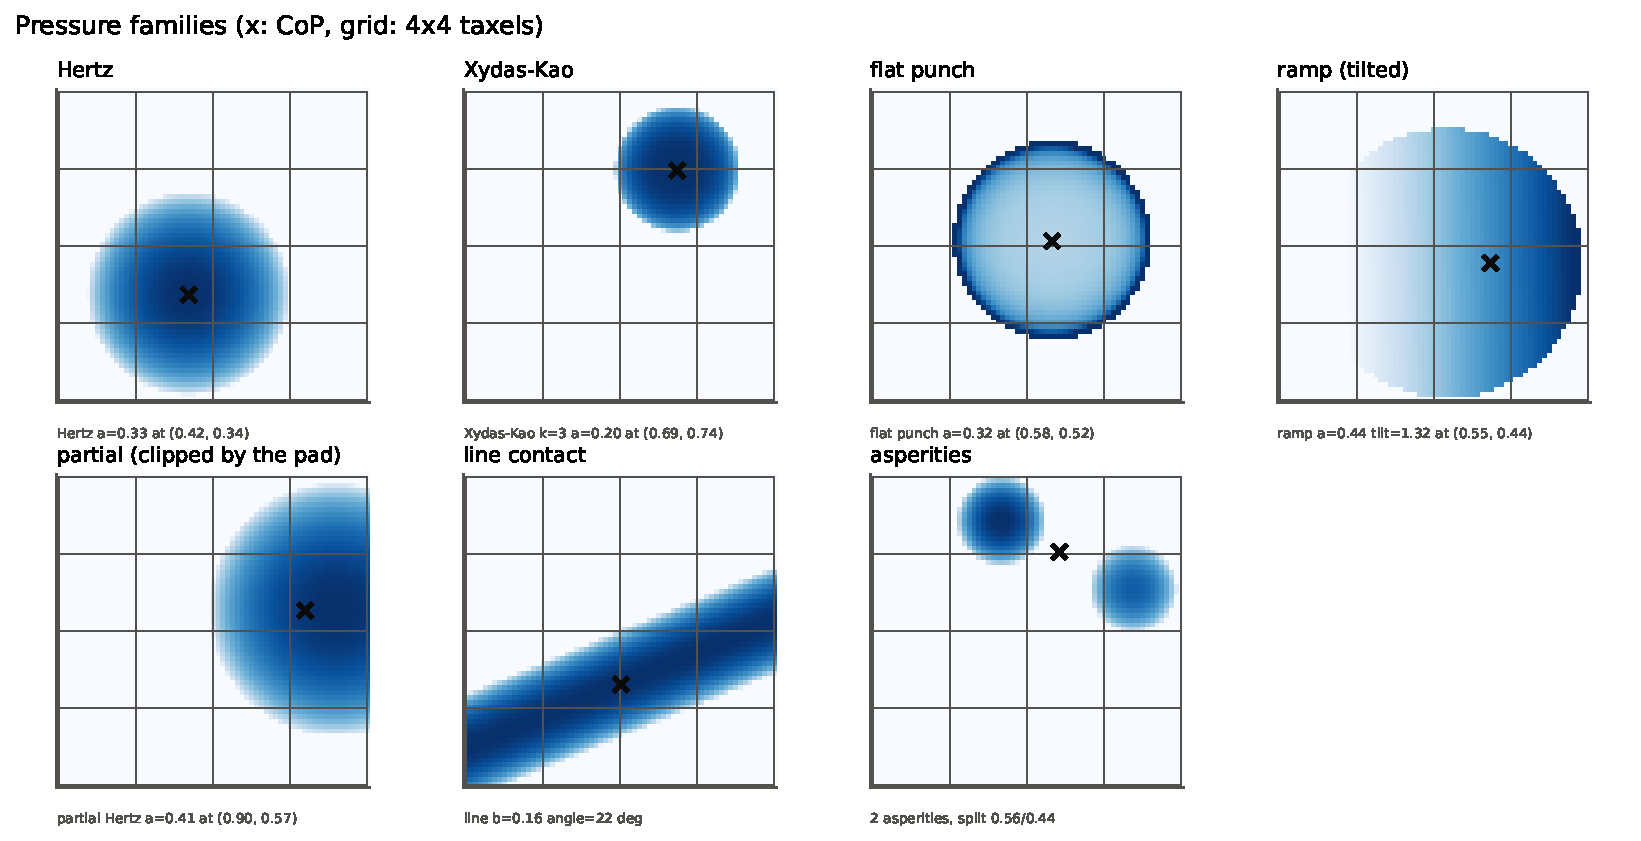
\includegraphics[width=\linewidth]{fields.pdf}
\caption{One field per family, with $4\times4$ taxels and the CoP (\code{examples/06\_fields.py}).}
\label{fig:fields}
\end{figure}

\subsection{F1: guaranteed and possible wrench sets}
\label{sec:F1}
\paragraph{Question.} What do the three measurement models guarantee and allow on a contact outside the parametric families (Q2, Q3)?
\paragraph{Protocol.} A partial, tilted contact (ramp clipped by the pad edge). The $(f_{T,1},\tau)$ slice of the true set $\X(\nu_N)$ is compared
with $\X^-$ and $\X^+$ for $\M_0$, $\M_F$, $\M_T$ at $4\times4$ and $16\times16$ taxels, with the torque about the true CoP for all three models
(\code{examples/07\_wrench\_sets.py}).
\paragraph{Result.} Figure~\ref{fig:F1}. The $\M_0$ guaranteed set is the force segment: no torsion about the CoP is guaranteed
(Corollary~\T{cor:coarse_inner}), and its possible set is wide. Taxel measurements give guaranteed sets with nonzero torsion, which close in on the
true set at $16\times16$. $\M_T$ is much tighter than $\M_F$: mean widths 0.129 ($\M_F$) and 0.039 ($\M_T$) at $4\times4$, 0.032 and 0.009 at
$16\times16$ (0.107 for $\M_0$).

\begin{figure}[tbp]
\centering
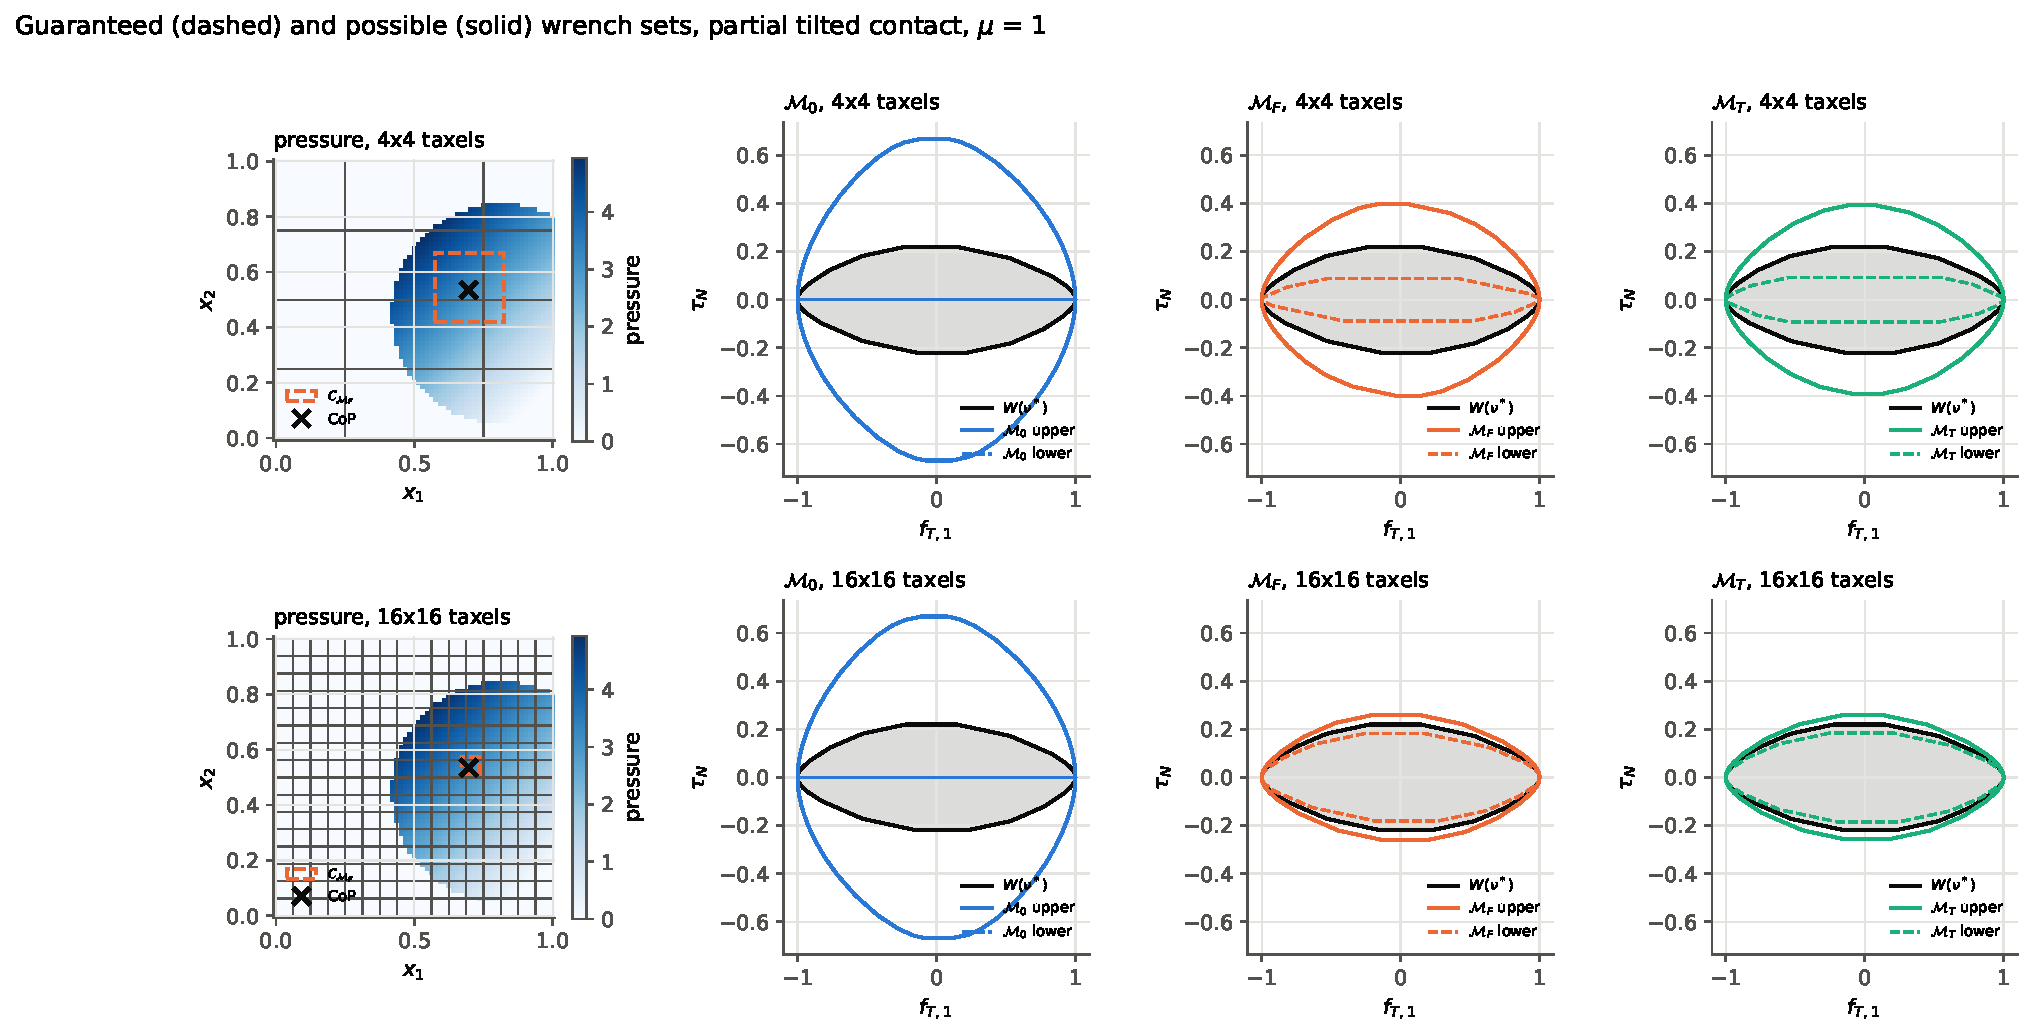
\includegraphics[width=\linewidth]{wrench_sets.pdf}
\caption{F1. True $\X(\nu_N)$ (grey), possible set $\X^+$ (solid) and guaranteed set $\X^-$ (dashed) for $\M_0$, $\M_F$, $\M_T$ on a partial tilted
contact, torque about the true CoP; rows: $4\times4$ and $16\times16$ taxels.}
\label{fig:F1}
\end{figure}
\paragraph{Interpretation.} An F/T sensor cannot support a torsional grasp decision, however accurate it is; distributed sensing is necessary,
and resolution decides how much of the true capacity can be used.

\subsection{F2: resolution and the value of measuring the CoP}
\label{sec:F2}
\paragraph{Question.} How do the bounds tighten with resolution, and what does the CoP add (Q2, Q3)?
\paragraph{Protocol.} Population of 21 fields, $k\times k$ taxels with $k=1,2,4,\dots,32$ (a dyadic chain, so the bounds tighten monotonically,
Proposition~\T{prop:taxel_refinement_MF}), two twists about the true CoP of each field: the unit rotation $q=(0,0,1)$ and a mixed twist
$q\propto(1,0,1/0.2)$ that balances force and torque at a lever of 0.2 pad sides (\code{examples/08\_resolution.py}). All bounds are exact. The gap
is compared with Proposition~\T{prop:taxel_resolution_MT} and Theorem~\T{thm:rate}.
\paragraph{Result.} Table~\ref{tab:F2} and Figure~\ref{fig:F2}.
\begin{itemize}
    \item For the rotation about the CoP, the median $\M_T$ lower bound rises from 0 (one taxel: Corollary~\T{cor:coarse_inner}) to 0.30 of the true
    support at $2\times2$, 0.68 at $8\times8$, 0.83 at $16\times16$ and 0.92 at $32\times32$; the upper bound falls from about 3 to 1.09.
    \item For the mixed twist, $\M_T$ guarantees 0.72 already with one taxel, and 0.96 at $32\times32$. $\M_F$ guarantees nothing with one taxel and only
    0.31 at $2\times2$: without the CoP, the center of rotation of the twist may lie under the load.
    \item The gap $(\overline h-\underline h)/(\mu|b|f_N)$ decreases linearly with the maximal taxel diameter and stays below the bound of
    Proposition~\T{prop:taxel_resolution_MT}, which holds for both models. From $4\times4$ on, each refinement divides the median $\M_F$ gap by
    $1.97$--$2.00$ (largest ratio over the fields 0.57, 0.53 and 0.505 for the three steps), as predicted by Theorem~\T{thm:rate}, and the median $\M_F$ gap is
    0.86--0.90 of the bound, inside the predicted range $[1/\sqrt2,1]$. The $\M_T$ gap shrinks at the same rate (median ratios 0.47--0.52).
    \item For the rotation about the CoP, measuring the CoP narrows the bounds by 12\% at $2\times2$ and by 2--8\% from $4\times4$ on. For the mixed
    twist it narrows them by 30--34\% at every resolution from $2\times2$ to $32\times32$ (46\% with one taxel).
\end{itemize}

\begin{table}[tbp]
\centering\small
\begin{adjustbox}{max width=\linewidth}\begin{tabular}{@{}lcccccc@{}}
\toprule
& \multicolumn{3}{c}{rotation about the CoP, $q=(0,0,1)$} & \multicolumn{3}{c}{mixed $q\propto(1,0,1/0.2)$ about the CoP} \\
\cmidrule(lr){2-4}\cmidrule(l){5-7}
taxels & $\M_T$ lower / upper & $\M_F$ lower / upper & CoP gain & $\M_T$ lower / upper & $\M_F$ lower / upper & CoP gain \\
\midrule
$1\times1$ & 0.00 / 2.97 & 0.00 / 3.94 & 23\% & 0.72 / 2.33 & 0.00 / 3.13 & 46\% \\
$2\times2$ & 0.30 / 2.48 & 0.18 / 2.74 & 12\% & 0.75 / 1.99 & 0.31 / 2.28 & 31\% \\
$4\times4$ & 0.48 / 1.78 & 0.48 / 1.81 & 3\% & 0.78 / 1.52 & 0.54 / 1.62 & 30\% \\
$8\times8$ & 0.68 / 1.39 & 0.68 / 1.39 & 2\% & 0.85 / 1.23 & 0.73 / 1.30 & 31\% \\
$16\times16$ & 0.83 / 1.19 & 0.83 / 1.19 & 2\% & 0.92 / 1.11 & 0.86 / 1.14 & 31\% \\
$32\times32$ & 0.92 / 1.09 & 0.91 / 1.09 & 8\% & 0.96 / 1.05 & 0.92 / 1.07 & 33\% \\
\bottomrule
\end{tabular}\end{adjustbox}
\caption{F2: median bound / true support over 21 fields (exact bounds). CoP gain: median of
$(\text{width}_{\M_F}-\text{width}_{\M_T})/\text{width}_{\M_F}$.}
\label{tab:F2}
\end{table}

\begin{figure}[tbp]
\centering
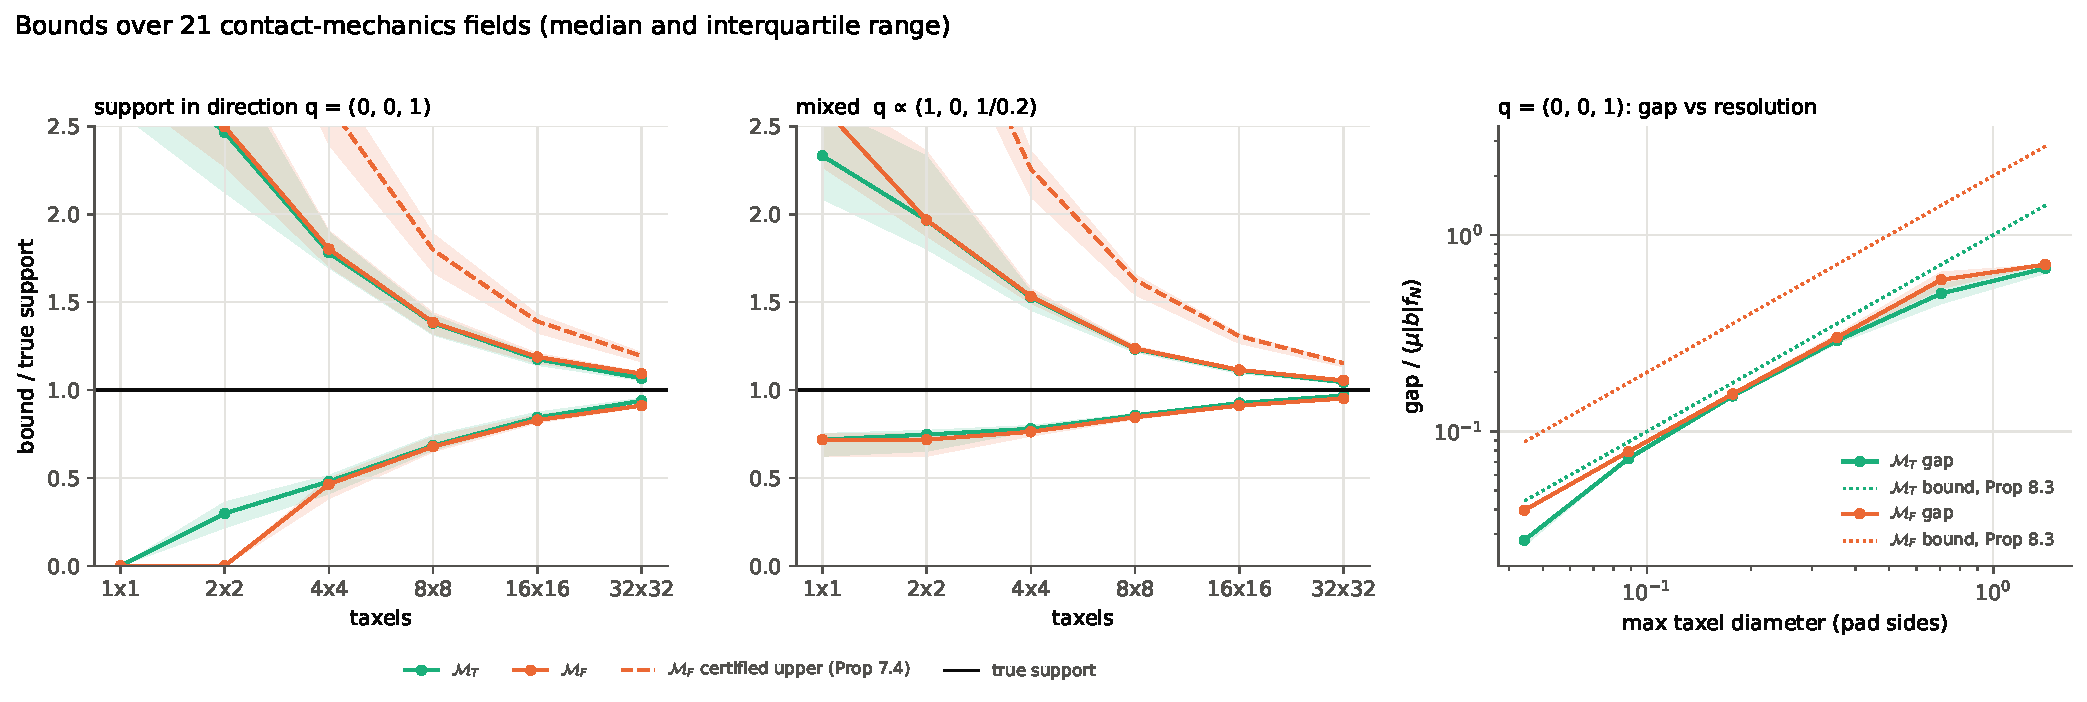
\includegraphics[width=\linewidth]{resolution.pdf}
\caption{F2. Bound / true support against resolution for $\M_T$ and $\M_F$ (median and interquartile band over the population), and the gap against
the maximal taxel diameter with the bound of Proposition~\T{prop:taxel_resolution_MT} (both models).}
\label{fig:F2}
\end{figure}
\paragraph{Interpretation.} Resolution is what makes torsion certifiable: from a guaranteed zero with an F/T sensor to more than 80\% of the true torsional
support at $16\times16$. The rate is the one predicted by Theorem~\T{thm:rate}: each halving of the taxel size halves the gap, and the bound of
Proposition~\T{prop:taxel_resolution_MT} is attained up to the factor of the theorem, so it is a usable design rule for sensor resolution. The value
of the CoP depends on the twist. For a rotation about the CoP itself, the taxel forces already locate the load well, and the CoP adds little beyond
$2\times2$. For a twist that combines force and torque, the CoP fixes the lever arm, and measuring it removes about a third of the width at every
resolution.
\paragraph{Changes from the previous version of this report.} The previous version took torques about the CoP of each candidate measure. Its $\M_T$
and $\M_0$ values are unchanged (they are the same quantities, by Lemma~\T{lem:varignon}), but its $\M_F$ columns bounded a twist that moved with each
candidate's CoP; they were tighter for the mixed twist (lower bound 0.72 at one taxel) and suggested that the CoP adds little at intermediate
resolution. That formulation is no longer used (Remark~\T{rem:MF_cop}). The previous study also used a $65\times65$ support grid; its 25--30\% CoP
gain at $32\times32$ was largely an effect of that grid (2 grid spacings per taxel), which the $129\times129$ grid removes.

\subsection{F3: certification versus plug-in estimation}
\label{sec:F3}
\paragraph{Question.} Is a plug-in estimate safe (Q4)?
\paragraph{Protocol.} Same population and directions (\code{examples/09\_plugin.py}): plug-in / true, and certified lower bound / true for $\M_T$ and $\M_F$.
\paragraph{Result.} Figure~\ref{fig:F3}. The plug-in support value, evaluated at the same twist, exceeds the truth for every field at every
resolution for the rotation about the CoP, and for all but one field (95\%) at $2\times2$ for the mixed twist. The worst overestimate for the rotation
is $\times2.6$ at $2\times2$, $\times1.47$ at $4\times4$, $\times1.11$ at $8\times8$ and $\times1.03$ at $16\times16$ (mixed twist: $\times1.87$, 1.15,
1.04, 1.01). The certified lower bounds are below the truth by construction (medians as in Table~\ref{tab:F2}).

\begin{figure}[tbp]
\centering
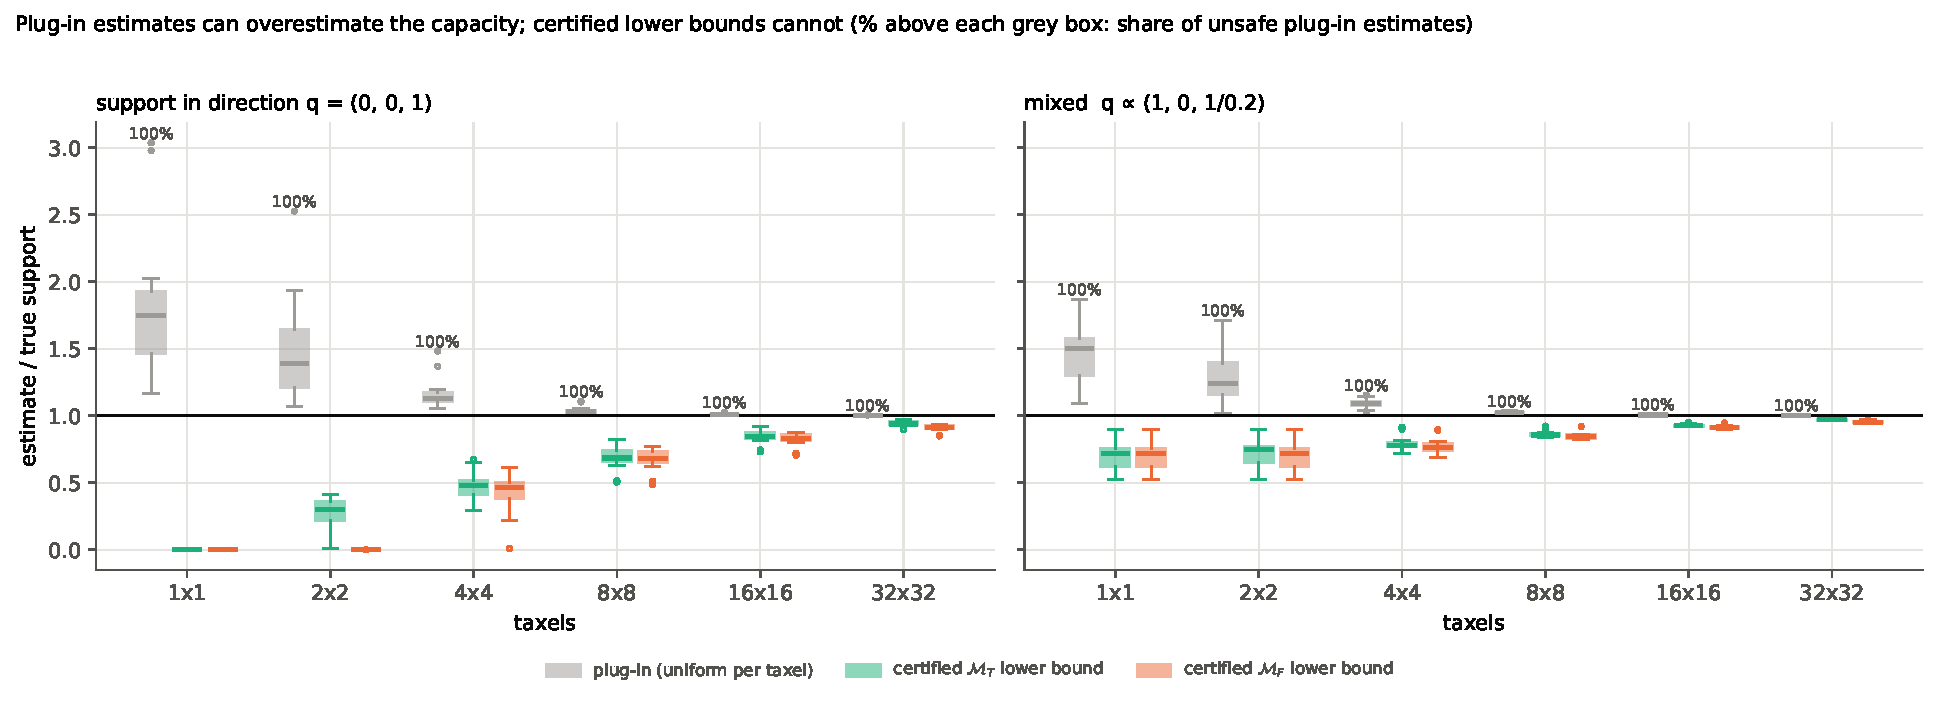
\includegraphics[width=\linewidth]{plugin.pdf}
\caption{F3. Plug-in / true (grey) and certified lower bound / true ($\M_T$ green, $\M_F$ orange) against resolution; the percentage is the share of
fields where the plug-in overestimates.}
\label{fig:F3}
\end{figure}
\paragraph{Interpretation.} The integrand $g$ is convex in $x$ (Lemma~\T{lem:integrand}), so load spread out carries more torsion than the same
load concentrated at its centroid. A plug-in estimate spreads each taxel force over the whole cell, including parts the real contact does not
touch (the contact edge, partial contacts), and is therefore biased toward overestimation, most strongly in torsion and at coarse resolution.
The bias shrinks with resolution and changed sign in one case only, so a plug-in estimate needs a margin tuned on data; the
certificate needs none. This is the comparison the closed loop repeats (Section~\ref{sec:S3}).

\subsection{Certified load factor and runtime}
\label{sec:loadfactor}
\paragraph{Question.} Support values describe the sets; a controller needs the capacity along a load. How tight and how fast are the certified
and upper load factors (Q2--Q4)?
\paragraph{Protocol.} Same population; loads $w$ about the pad centre: a pure torque and a force at lever 0.2; $\underline s/s^\star$ and
$\overline s/s^\star$ for $\M_T$ and $\M_F$, the plug-in load factor, and the solve time of one certificate (\code{examples/10\_load\_factor.py}).
\paragraph{Result.} Table~\ref{tab:LF} and Figure~\ref{fig:loadfactor}.

\begin{table}[tbp]
\centering\small
\begin{adjustbox}{max width=\linewidth}\begin{tabular}{@{}lcccccccc@{}}
\toprule
& \multicolumn{4}{c}{pure torque $w=(0,0,1)$} & \multicolumn{4}{c}{force at lever 0.2, $w=(1,0,0.2)$} \\
\cmidrule(lr){2-5}\cmidrule(l){6-9}
taxels & $\M_T$ & $\M_F$ & $\M_T$ upper & plug-in (share $>1$) & $\M_T$ & $\M_F$ & $\M_T$ upper & plug-in (share $>1$) \\
\midrule
$1\times1$ & 0.00 & 0.00 & 2.93 & 1.75 (100\%) & 0.00 & 0.00 & 1.34 & 1.22 (81\%) \\
$2\times2$ & 0.24 & 0.00 & 2.46 & 1.39 (100\%) & 0.39 & 0.00 & 1.33 & 1.15 (95\%) \\
$4\times4$ & 0.46 & 0.43 & 1.79 & 1.14 (100\%) & 0.61 & 0.47 & 1.21 & 1.06 (95\%) \\
$8\times8$ & 0.68 & 0.68 & 1.38 & 1.04 (100\%) & 0.80 & 0.75 & 1.14 & 1.02 (95\%) \\
$16\times16$ & 0.83 & 0.83 & 1.19 & 1.01 (100\%) & 0.91 & 0.87 & 1.08 & 1.01 (95\%) \\
$32\times32$ & 0.92 & 0.91 & 1.09 & 1.00 (100\%) & 0.96 & 0.93 & 1.04 & 1.00 (95\%) \\
\bottomrule
\end{tabular}\end{adjustbox}
\caption{Load factors: median certified / true and upper / true load factor ($\M_T$; $\M_F$ upper: 3.23, 2.46, 1.80, 1.38, 1.19, 1.09 for the torque and
1.44, 1.44, 1.37, 1.23, 1.12, 1.06 for the lever load), and plug-in / true over 21 fields, with the share of fields where the plug-in overestimates.
Solve time of one certificate (one pad): 9--11\,ms up to $4\times4$, 12--13\,ms at $8\times8$, 22--24\,ms at $16\times16$, 74--77\,ms at
$32\times32$.}
\label{tab:LF}
\end{table}

\begin{figure}[tbp]
\centering
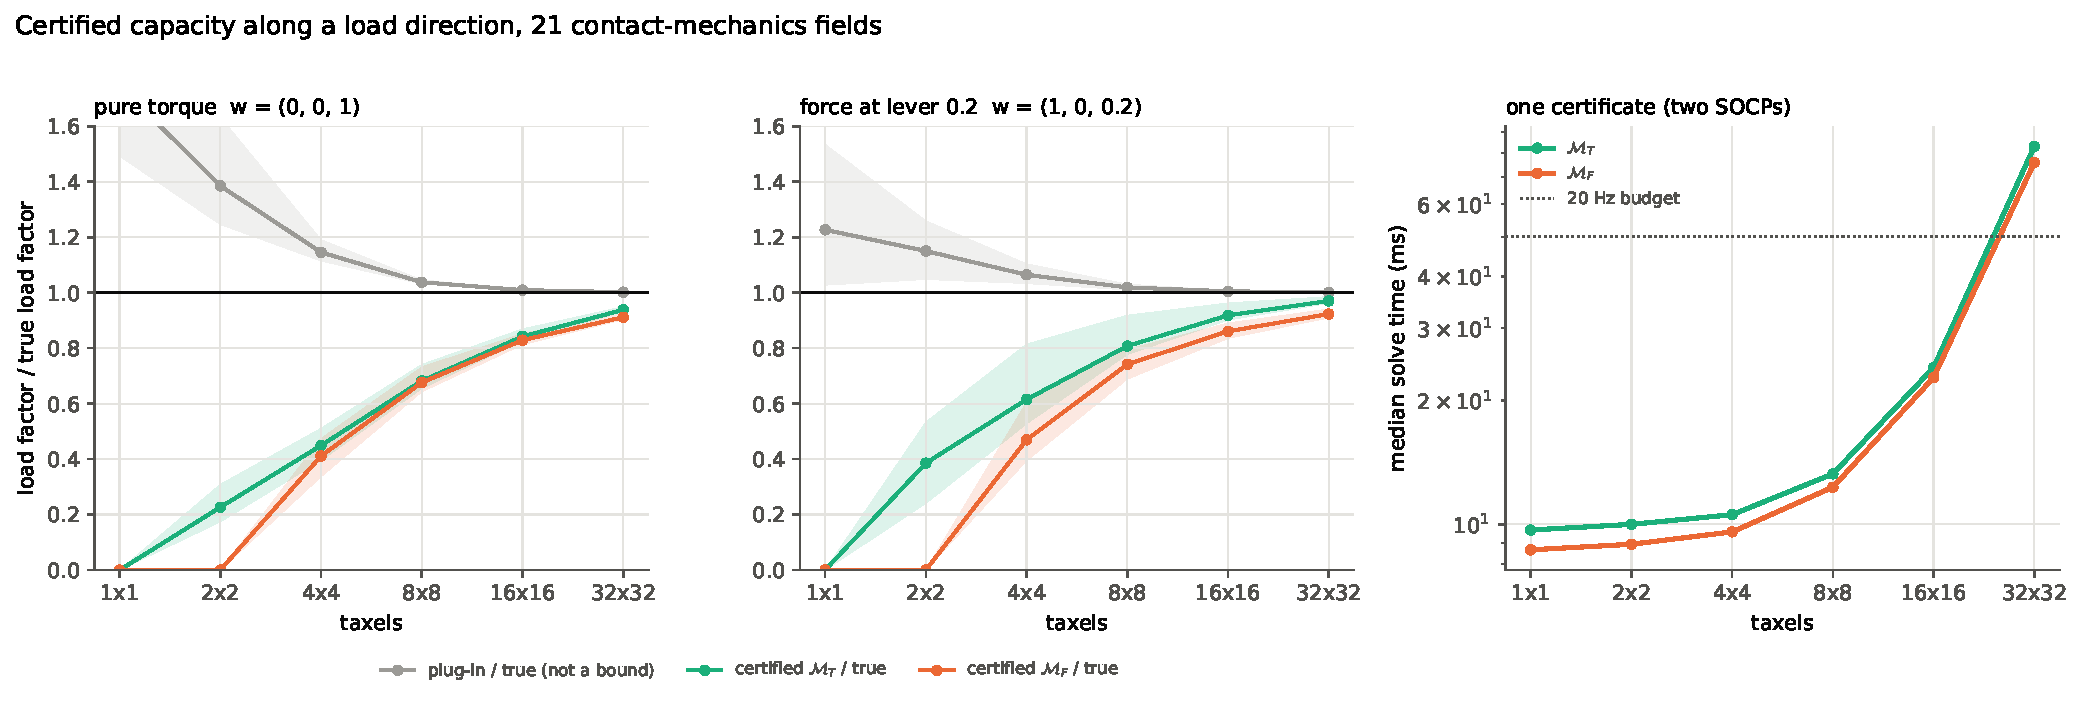
\includegraphics[width=\linewidth]{load_factor.pdf}
\caption{Certified (solid) and upper (dashed) load factor / true load factor for $\M_T$ and $\M_F$ against resolution (median and interquartile range),
plug-in / true, and solve time of one certificate.}
\label{fig:loadfactor}
\end{figure}
\paragraph{Interpretation.} The certified load factor behaves like the support bounds: from zero guaranteed torque with an F/T sensor to 83\% of the true
torque capacity at $16\times16$, within tens of milliseconds, fast enough for a 20\,Hz control loop. With a force at a lever arm the one-taxel
certificate is also zero, because the load contains a torque about $o$. Without the CoP ($\M_F$) the certificate is zero at $2\times2$ and lags $\M_T$
by up to 14 points for loads with a force component, where the unknown CoP shifts the lever arm. The plug-in load factor overestimates in all
fields for a pure torque and in 81--95\% for the lever load. The values are those of the previous version of this report up to the finer support
grid (the certified load factor did not change with the fixed-frame formulation, which it already used). Pure-torque capacity is $\inf_ah((a,1))$, slightly below the support value
$h((0,0,1))$ of F2, which is why the load-factor ratios at $2\times2$ (0.24) are below the support ratios (0.30).
\paragraph{Decision band.} The two factors bracket the true capacity: a load is surely held below $\underline s$ and surely lost above $\overline s$
(Proposition~\T{prop:load_factor}(v)). For a pure torque with $\M_T$, the undecided band shrinks from $[0.24,2.46]$ times the true capacity at
$2\times2$ to $[0.83,1.19]$ at $16\times16$ and $[0.92,1.09]$ at $32\times32$. A controller can therefore also detect, from the measurement alone, that a
demanded load exceeds what any compatible contact could carry: for the median field at $16\times16$, any pure torque more than 19\% above the true
capacity. In the closed loop of S3 and S4
only the certified factor was used.

% =====================================================================================================
\section{Drake simulation studies}
\label{sec:drake}

\subsection{Why Drake, and what it can test}
\label{sec:simulator}
Drake's hydroelastic contact computes a contact surface with a pressure field; in its discrete solvers each face of that surface is a compliant
point contact at its centroid, with force $A_fp_f$ and Coulomb friction, and torsion emerges from the distributed points
\citep{masterjohn2022velocity}. Two consequences:
\begin{itemize}
    \item For frozen normal forces, the static capacity of a simulated contact \emph{is} the support function of the theory on a discrete field.
    The true capacity of every simulated state is therefore known exactly, and a pressure field is available at every step, which hardware
    cannot provide.
    \item The dynamics are not those of the theory: compliance, regularized friction, time stepping, actuator lag and load dynamics. These are
    what the simulation tests, together with the sensing pipeline.
\end{itemize}
Drake cannot validate Coulomb friction on a gel, and a slip in simulation is a slip of Coulomb's law as Drake regularizes it. Tactile simulators
were considered and not used: the mechanics-based ones also implement Coulomb friction, so checking slip against the bounds would be circular,
and none would test the silicone behaviour reported by \citet[§3]{howe1996practical}. MuJoCo was excluded because its torsional friction is a
lumped coefficient with no pressure field.

\paragraph{Sensing.} A pad's measurement is read from the contact surface: each face is one point load (pressure $\times$ area at its centroid);
taxel forces are the sums over the faces whose centroids fall in each taxel of a $k\times k$ grid on a $32\times32$\,mm footprint centred at the
reference point $o$; the CoP is the force-weighted mean. Faces on non-parallel side walls are excluded and monitored; states with more than
0.5\% of the force on side walls or outside the footprint are rejected. All wrenches are expressed in the grasp plane in common coordinates
$u=(z,x)$, torques about the grip axis $y$, reference $o=0$, loads $w=(f_z,f_x,\tau_y)$. The certificates of S2--S4 were always computed about this
fixed point, so the fixed-frame formulation of the theory leaves S1--S4 unchanged.

\subsection{S1: contact read-out}
\label{sec:S1}
\paragraph{Question.} Does the read-out of Drake's contact surface give the forces Drake applies (Q1)?
\paragraph{Protocol.} A rigid block resting on a compliant pad (\code{sim/smoke\_contact.py}).
\paragraph{Result.} The sum of the face forces is 4.8957\,N, against Drake's resultant 4.9045\,N and the weight 4.9050\,N (98 faces); the CoP is
within 0.03\,mm of the block's placement. The true pure-torque capacity of the contact (17.480\,N\,mm) is close to its support value
$h(0,0,1)=17.485$\,N\,mm, and to the capacity of a uniform $12\times12$\,mm square (18.016\,N\,mm).
\paragraph{Interpretation.} The face read-out is a faithful measurement of the simulated contact (0.2\% below Drake's resultant), so the taxel
forces of the later studies are those of the simulated pressure field.

\subsection{S2: break-away against the certificate, and solver sensitivity}
\label{sec:S2}
\paragraph{Question.} Does a simulated grasp break away at its true load factor, and does the certified load factor stay below the observed
break-away (Q1)? Is the answer robust to the simulator's settings?
\paragraph{Protocol.} A rigid bar squeezed between two flat compliant pads ($20\times16$\,mm, about 7.9\,N each, no gravity). A force along $z$ is
ramped slowly at a 30\,mm lever arm in the mid-plane, so the load direction $w=(1,0,-0.03)$ combines shear and torque about the grip axis. The
observed break-away $s_{\rm obs}$ is the force at which the bar speed exceeds 1\,mm/s; $s_{\rm true}$ is the exact load factor of Drake's faces just
before slip; the certificate is $\M_T$ $16\times16$ on both pads. The sweep varies the discrete contact solver, its stiction tolerance, the time
step, ramp rate, mesh size, detection threshold and pad modulus (\code{sim/sweep\_breakaway.py}).
\paragraph{Result.} Table~\ref{tab:S2}.

\begin{table}[tbp]
\centering\small
\begin{adjustbox}{max width=\linewidth}\begin{tabular}{@{}lcc@{}}
\toprule
Setting & $s_{\rm obs}/s_{\rm true}$ & certified $/s_{\rm obs}$ \\
\midrule
lagged, stiction tolerance $10^{-6}$\,m/s (reference) & 1.001 & 0.915 \\
time step $2.5\cdot10^{-4}$ / ramp 0.5\,N/s / mesh 0.5\,mm / threshold 0.3\,mm/s / modulus $2\cdot10^6$ & 0.992--1.001 & 0.915--0.923 \\
stiction tolerance $10^{-5}$ & 0.997 & 0.918 \\
\textbf{stiction tolerance $10^{-4}$ (Drake default)} & \textbf{0.893} & \textbf{1.025} (violated) \\
similar, stiction $10^{-6}$ & 1.001 & 0.915 \\
\textbf{SAP (automatic regularization)} & \textbf{1.360} & 0.673 \\
\bottomrule
\end{tabular}\end{adjustbox}
\caption{S2: break-away of the bar against the true and certified load factors, over solver settings. Side walls carried 0.00\% of the force.}
\label{tab:S2}
\end{table}
\paragraph{Interpretation.}
\begin{itemize}
    \item With the lagged or similar solvers and a stiction tolerance of at most $10^{-5}$\,m/s, the bar breaks away within 1\% of the ideal Coulomb
    capacity, insensitive to time step, ramp rate, mesh and stiffness, and the certificate stays below it (0.915--0.923 at $16\times16$; about
    0.5 with one pad unsensed). Two-pad additivity (Proposition~\T{prop:load_factor}(vi)) holds in this setting.
    \item Drake's default tolerance makes points near the rotation centre creep below full friction, so the bar breaks away at 89\% of its
    capacity and a sound certificate \emph{appears} violated. SAP holds 36\% above the Coulomb capacity although its normal forces match the
    pressure field within 0.6\%; the cause is unexplained and SAP is excluded.
    \item A simulator's friction regularization can contradict a Coulomb guarantee. S3 and S4 use the lagged solver with stiction tolerance
    $10^{-6}$, and the setting must be reported with any simulation result.
    \item Runtime: a two-pad $\M_T$ $16\times16$ certificate takes about 41\,ms serially (one pad: 22\,ms), within a 20\,Hz control budget.
\end{itemize}

\subsection{S3: closed-loop certified grip control}
\label{sec:S3}
\paragraph{Question.} If a controller squeezes just enough to keep the demanded load certified, does the grasp hold, at what squeeze, and how does
this compare with nominal estimators whose margins are tuned on data (Q5)?

\paragraph{Scene.} A rigid bar ($150\times20\times60$\,mm, gravity off) moves on a planar joint (translations $x,z$, rotation about the grip axis $y$)
between two compliant pads (hydroelastic modulus $5\cdot10^5$\,Pa, $\mu=0.8$), each on a prismatic joint and pushed with the same squeeze, which
follows the command through a first-order filter ($\tau=50$\,ms, the gripper bandwidth). Three pad families, both pads drawn independently within
the family: \emph{dome} (ellipsoid, Hertz-like field whose area grows with the squeeze), \emph{tilted} box (ramp field or partial edge contact) and
\emph{flat} box (near-uniform field, the control case). Solver: lagged, stiction tolerance $10^{-6}$.

\paragraph{Loads.} The demanded grasp wrench is $D(t)\,w(t)$ in the grasp plane. 20\% of the seeds demand a pure torque, the others a force at a
lever of 2--6 RMS contact radii, so that torsion binds (the peak squeeze is at least three times the shear-only value). Scenario~A (the
hardware task): $D$ ramps to $D_{\max}$ over 3\,s along a fixed $w$, then holds for 1\,s. Scenario~B: $D$ oscillates between 0.3 and 1 times
$D_{\max}$ while the lever swings between 0 and its maximum over 7\,s, so the binding direction changes. 30 seeds per scenario.

\paragraph{Controller (identical for every method).} Every 50\,ms the method estimates the load factor $\hat s$ of the current contact along $w$ and
commands
\begin{align}
    f_{\rm cmd}=\operatorname{clip}\!\left(f_{\rm meas}\,\frac{D\,(1+m)}{\hat s},\;F_{\min},\;f_{\max}\right),
\end{align}
with $F_{\min}=1$\,N, decreases limited to 2\% per cycle, and $D$, $w$ taken 150\,ms ahead (one control period plus about two filter time constants;
the load profile is known). In B, the larger of the commands for the current and the upcoming load is used. Three declared heuristics lie
outside the theory: (i) capacity scales linearly with squeeze ($\hat s/f_{\rm meas}$ is a capacity per newton; on domes it grows with squeeze, so the
update is conservative there); (ii) the relaxation limit; (iii) the load preview. A certificate is sound for the measured state only.

\paragraph{Force budget and flag.} Pushing a thin compliant pad past about half its thickness flattens and then reverses the hydroelastic
force--depth law. In a pilot, the coarse $2\times2$ certificate at $m=1$ commanded 46\,N on a dome while the measured squeeze fell from 44.6 to
25\,N, and the bar slipped. The command is therefore clipped at a per-seed budget $f_{\max}$, the static squeeze at 50\% of the pad's
semi-thickness (18--76\,N), and an episode is \emph{flagged} at the first cycle where the requested squeeze exceeds it.

\paragraph{Free object.} In a pilot with a free bar, pads whose normal-force centres did not line up created a couple about an in-plane axis that
opposite tangential forces at the two faces had to balance; the oracle slipped at a 5\% margin with a bar tilt of about 1.6$^\circ$. The planar
certificate does not account for this internal load: Proposition~\T{prop:load_factor}(vi) assumes the out-of-plane components are balanced without
friction. The planar joint enforces that assumption in the study; with a real free object it is a limitation (Remark~\T{rem:load_factor}).

\paragraph{Design.} 30 seeds $\times$ 2 scenarios $\times$ (3 oracle margins + 10 methods $\times$ 6 margins,
$m\in\{0,0.05,0.1,0.25,0.5,1\}$) $=3780$ episodes (1.8\,h on 22 processes); none was rejected by the side-wall and footprint filters.

\paragraph{Result 1: outcomes.} Table~\ref{tab:S3} (scenario A; B is within a few points) and Figure~\ref{fig:S3}.

\begin{table}[tbp]
\centering\small
\begin{adjustbox}{max width=\linewidth}\begin{tabular}{@{}lcccc@{}}
\toprule
Method & $m=0$ & $m=0.05$ ($m_{\rm dyn}$) & $m=0.25$ & $m=1$ \\
\midrule
oracle ($m=0$ / 0.05 / 0.1) & 3/0/97 $\cdot$ 0.96 & 100/0/0 $\cdot$ 1.00 & (0.1) 100/0/0 $\cdot$ 1.05 & \\
certified $\M_T$ $2\times2$ & 87/13/0 $\cdot$ 2.95 & 83/17/0 $\cdot$ 3.10 & 70/30/0 $\cdot$ 3.69 & 7/93/0 $\cdot$ 3.85 \\
certified $\M_T$ $4\times4$ & 93/7/0 $\cdot$ 2.37 & 93/7/0 $\cdot$ 2.48 & 93/7/0 $\cdot$ 2.94 & 47/53/0 $\cdot$ 5.87 \\
certified $\M_T$ $8\times8$ & 100/0/0 $\cdot$ 1.33 & 100/0/0 $\cdot$ 1.40 & 100/0/0 $\cdot$ 1.66 & 93/7/0 $\cdot$ 2.63 \\
certified $\M_T$ $16\times16$ & 100/0/0 $\cdot$ 1.13 & \textbf{100/0/0 $\cdot$ 1.18} & 100/0/0 $\cdot$ 1.40 & 100/0/0 $\cdot$ 2.20 \\
certified $\M_F$ $16\times16$ & 100/0/0 $\cdot$ 1.17 & 100/0/0 $\cdot$ 1.23 & 100/0/0 $\cdot$ 1.46 & 100/0/0 $\cdot$ 2.26 \\
certified, one pad sensed & 100/0/0 $\cdot$ 2.30 & 97/3/0 $\cdot$ 2.40 & 83/17/0 $\cdot$ 2.80 & 60/40/0 $\cdot$ 4.72 \\
plug-in $4\times4$ & 3/0/97 $\cdot$ 0.97 & 13/0/87 $\cdot$ 0.97 & 60/0/40 $\cdot$ 1.11 & 97/0/3 $\cdot$ 1.70 \\
plug-in $16\times16$ & 23/0/77 $\cdot$ 0.96 & 77/0/23 $\cdot$ 0.99 & 100/0/0 $\cdot$ 1.16 & 100/0/0 $\cdot$ 1.85 \\
F/T + contact mask & 0/0/100 & 50/0/50 $\cdot$ 0.99 & 100/0/0 $\cdot$ 1.16 & 100/0/0 $\cdot$ 1.83 \\
uniform over pad (F/T only) & 0/0/100 & 0/0/100 & 0/0/100 & 73/0/27 $\cdot$ 1.20 \\
\bottomrule
\end{tabular}\end{adjustbox}
\caption{S3, scenario A: success / infeasible / silent slip (\%) $\cdot$ median effort of the successes (squeeze / oracle at $m_{\rm dyn}$).}
\label{tab:S3}
\end{table}

\begin{figure}[tbp]
\centering
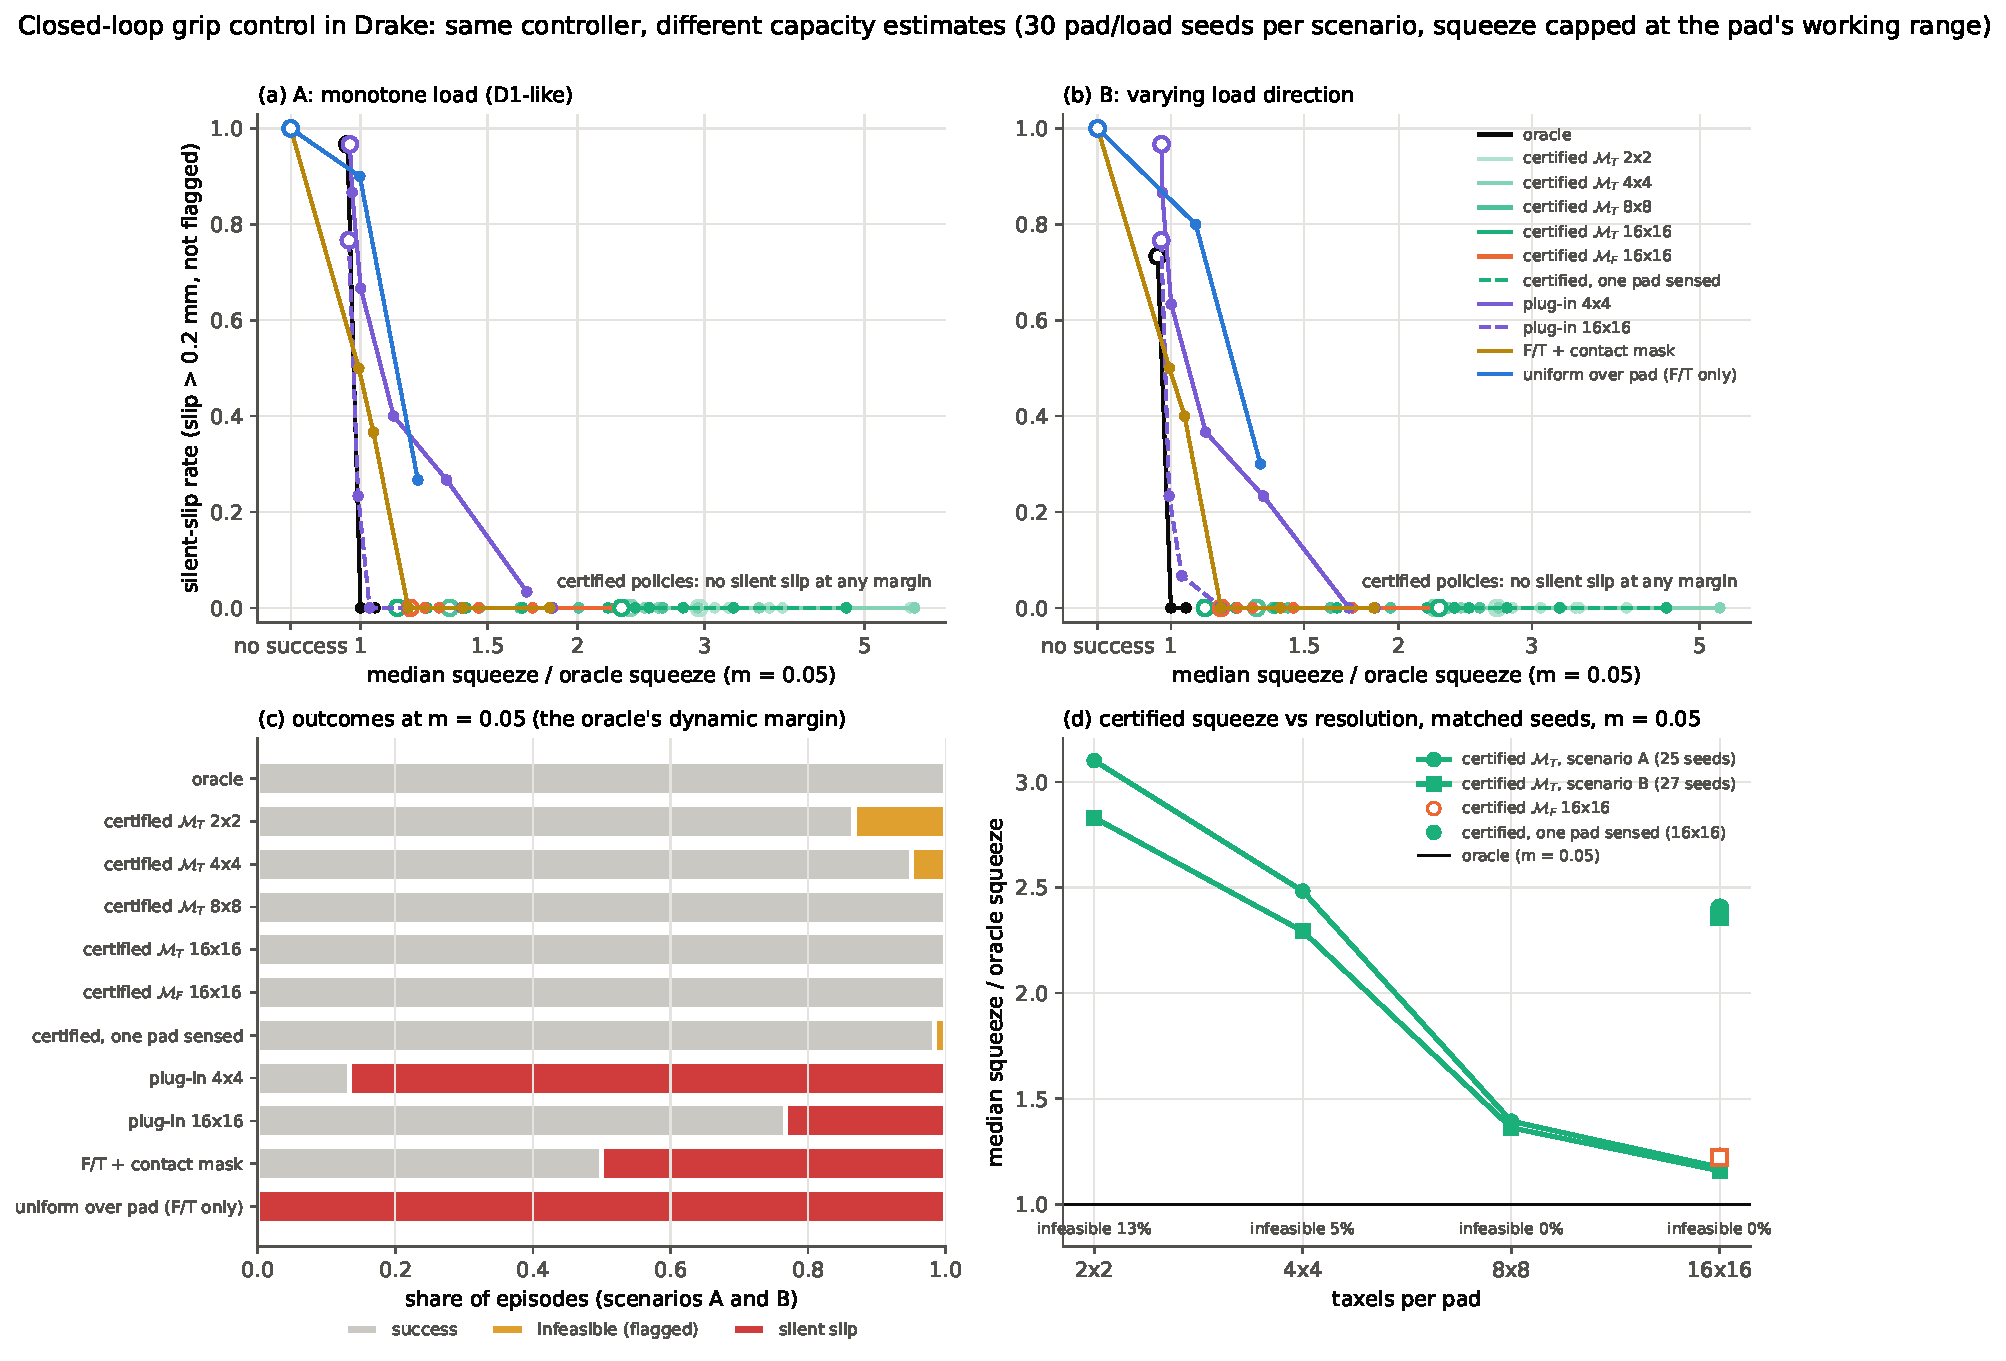
\includegraphics[width=\linewidth]{grip_pareto.pdf}
\caption{S3. (a, b) Silent-slip rate against median squeeze for every method and margin, scenarios A and B. (c) Outcomes at $m_{\rm dyn}$.
(d) Certified squeeze against resolution on matched seeds, with the infeasible rate.}
\label{fig:S3}
\end{figure}

\begin{itemize}
    \item \textbf{No certified silent slip:} 0 of 2160 certified episodes, at every margin, in both scenarios and all pad families; the largest slip
    was 0.08\,mm against the 0.2\,mm threshold. 228 certified episodes were flagged; none slipped afterwards. Since the certificate is
    conservative, a flag means ``cannot certify within the budget'', not ``will slip''.
    \item The nominal methods slip \emph{silently} whenever they slip: their estimate never asks for more than the budget.
    \item \textbf{Infeasibility is the cost of coarse resolution:} at $m_{\rm dyn}$, 13\% ($2\times2$), 5\% ($4\times4$) and 0\% ($8\times8$, $16\times16$) of
    the episodes, pooled over A and B. The flagged seeds have budgets from 18 to 76\,N, so the flags come from a high certified demand (large
    lever arms on coarse taxels), not only from small budgets.
    \item \textbf{F/T only fails} even at $m=1$ (27\% silent slips): the real contacts are smaller than the pad.
\end{itemize}

\paragraph{Result 2: effort on matched seeds.} Table~\ref{tab:S3matched}.

\begin{table}[tbp]
\centering\small
\begin{adjustbox}{max width=\linewidth}\begin{tabular}{@{}lcccccc@{}}
\toprule
& $2\times2$ & $4\times4$ & $8\times8$ & $16\times16$ & $\M_F$ $16\times16$ & one pad \\
\midrule
A (25 seeds) & 3.10 & 2.48 & 1.39 & 1.18 & 1.23 & 2.40 \\
B (27 seeds) & 2.83 & 2.29 & 1.36 & 1.16 & 1.22 & 2.36 \\
\bottomrule
\end{tabular}\end{adjustbox}
\caption{S3: median squeeze / oracle at $m_{\rm dyn}$ on the seeds where the oracle and all certified methods succeed.}
\label{tab:S3matched}
\end{table}

Resolution buys most of the efficiency: the certified squeeze falls from about 3 times the oracle at $2\times2$ to 1.18 at $16\times16$. Measuring the CoP
adds little at $16\times16$ ($\M_F$ 1.23). Sensing one pad only costs as much as dropping to about $4\times4$ on both pads (2.40): the unsensed pad's
unknown pressure is charged at its worst case.

\paragraph{Result 3: nominal margins, tuned then tested.} The margin of each nominal method is tuned as the smallest margin without silent slip on a
training set, then tested on held-out data, with two splits: by seed (tune on A seeds 0--14, test on A seeds 15--29 and on B), and by contact
geometry (tune on the flat pads of A, test on the curved pads, dome and tilted, of A and B). Table~\ref{tab:S3tuned}.

\begin{table}[tbp]
\centering\small
\begin{adjustbox}{max width=\linewidth}\begin{tabular}{@{}lll@{}}
\toprule
Method & tuned on A seeds 0--14 $\to$ test A 15--29; B & tuned on flat pads $\to$ test curved pads A; B \\
\midrule
plug-in $4\times4$ & no safe margin up to $m=1$ & $m=0.1$ $\to$ 100\%; 95\% \\
plug-in $16\times16$ & $m=0.1$ $\to$ 0\% (1.03 vs 1.20); 7\% (1.03 vs 1.16) & $m=0.05$ $\to$ 35\%; 35\% \\
F/T + contact mask & $m=0.25$ $\to$ 0\% (1.11 vs 1.20); 0\% (1.16 vs 1.16) & $m=0.05$ $\to$ 75\%; 75\% \\
uniform over pad & no safe margin up to $m=1$ & $m=1$ $\to$ 40\%; 45\% \\
\bottomrule
\end{tabular}\end{adjustbox}
\caption{S3: silent-slip rate on the test set at the tuned margin, and effort against certified $\M_T$ $16\times16$ at $m_{\rm dyn}$ (matched seeds).}
\label{tab:S3tuned}
\end{table}

\begin{itemize}
    \item \textbf{On a representative training set, tuned nominal methods are cheaper.} Plug-in $16\times16$ at $m=0.1$ needs 1.03 times the oracle
    squeeze against 1.16--1.20 for the certificate, but slips in 7\% of B; the contact-mask method at $m=0.25$ needs 1.11--1.16 and transfers from
    A to B without slip. The certificate costs 0--17\% more squeeze than the best tuned baseline (equivalently, the baseline needs 0--14\% less).
    \item \textbf{Under a shift of contact geometry, tuned margins fail.} Margins tuned on flat pads slip in 35\% (plug-in $16\times16$) to 75\%
    (contact mask) of the curved-pad episodes. The contact-mask method fails exactly where its uniform-pressure assumption is wrong: 100\% silent
    slip on domes at $m_{\rm dyn}$, 0\% on flat pads.
\end{itemize}

\paragraph{Result 4: the oracle at zero margin.} The oracle slips at $m=0$ (97\% in A, 73\% in B). The slips occur in the hold phase after the ramp
(median 3.05\,s, the ramp ends at 3\,s), where the loop converges to capacity / demand $\approx1.01$; during the ramp the preview keeps it near
1.04. At $m=0.02$, the oracle holds with 0.06\,mm of creep. A zero-margin decision therefore leaves no room for model error (the simulated break-away
matched the computed capacity only to 0.992--1.001 in S2): this is a boundary effect, not evidence that static admissibility is insufficient.

\paragraph{Interpretation.}
\begin{itemize}
    \item The certificate holds in closed loop, including on contacts far from any parametric family, and signals infeasibility before slip. The
    loop needs about 5\% of slack (the oracle's dynamic margin), which a certificate at $m_{\rm dyn}$ provides; the zero-failure result at $m=0$ of
    the certified methods relies on their conservatism and is not a dynamic guarantee.
    \item The value of certification is \emph{robustness, not efficiency}: no calibration set, an explicit infeasibility flag, and immunity to
    shifts of contact geometry. Its price at $16\times16$ is 16--18\% squeeze over the oracle and 0--17\% over the best tuned baseline.
    \item Decision time under the 22-process pool was 56--172\,ms for the certificates; serially, on frozen states, 14--45\,ms (two-pad $\M_T$
    $16\times16$ about 40\,ms), within 20\,Hz.
\end{itemize}

\subsection{S4: sensing delay and load rate}
\label{sec:S4}
\paragraph{Question.} The certificate concerns the measured state. How much sensing delay does the S3 loop tolerate, with the S3 margins and no
retuning (Q6)?

\paragraph{Where the delay acts.} Under linear scaling, $\hat s/f_{\rm meas}$ in the S3 command is a capacity per newton. It depends on the shape of the
pressure field, not on the squeeze level, and changes slowly, so a stale tactile state should matter little. The load is different: S3 knew
the load profile 150\,ms ahead, whereas in the hardware task (a cup being filled) the load is measured, late. The study therefore runs the same
controller in two information modes:
\begin{itemize}
    \item \textbf{P (load previewed):} the S3 loop; the tactile state and $f_{\rm meas}$ are $\Delta$ old.
    \item \textbf{M (load measured):} the load is also measured $\Delta$ late, with no preview: $D(t-\Delta)$ replaces $D(t+150\,{\rm ms})$.
\end{itemize}

\paragraph{Design.} Scenario A only (the hardware task); delays $\Delta\in\{0,25,50,100,200\}$\,ms (25--50\,ms: a 30--60\,fps vision-based tactile frame
plus processing; 100--200\,ms: a slow pressure reconstruction); load-rate factor 1, 2, 4 (ramp 3, 1.5, 0.75\,s); six methods at their S3 margins:
oracle, $\M_T$ $8\times8$, $\M_T$ $16\times16$ and one pad at $m_{\rm dyn}=0.05$, plug-in $16\times16$ at its tuned 0.1, contact mask at its tuned 0.25.
30 seeds; 5400 episodes, none rejected. The delayed state is sampled at the simulation's 5\,ms sub-steps. With $\Delta=0$ and preview, the episodes
reproduce S3 exactly. Not varied, with reasons: the control rate (a held command acts like extra delay, the $16\times16$ two-pad certificate needs
about 40\,ms so 50\,Hz is unrealistic, and changing the period also changes the preview horizon); a slower load (easier than nominal); scenario~B.
\textbf{Prediction stated before the run:} P flat; M degrading for every method, the oracle included.

\paragraph{Slip-onset diagnosis.} At the first step where the slip exceeds 0.05\,mm, the shortfall of the true capacity $s_{\rm true}$ of the current
contact against the applied demand $D_{\rm now}$ splits exactly against the last decision (sensed state, load $D$ certified, estimate $\hat s$,
command $f_{\rm cmd}$):
\begin{align}
    \ln\frac{D_{\rm now}}{s_{\rm true,now}}
    =\underbrace{\ln\frac{\hat s}{s_{\rm true}(\text{sensed})}}_{\text{estimate}}
    +\underbrace{\ln\frac{D_{\rm now}}{D}}_{\text{load}}
    +\underbrace{\ln\frac{\kappa_{\rm sensed}}{\kappa_{\rm now}}}_{\text{state}}
    +\underbrace{\ln\frac{f_{\rm cmd}}{f_{\rm now}}}_{\text{actuator}}
    +\underbrace{\ln\frac{\text{target}}{f_{\rm cmd}}}_{\text{slack}\,\le0}
    -\ln(1+m),
\end{align}
with $\kappa=s_{\rm true}/f$ the true capacity per newton and the slack due to the squeeze floor or the relaxation limit. The cause of a slip is
the largest of the four cause terms, or \emph{model} if the Coulomb capacity still exceeds the demand ($s_{\rm true,now}\ge D_{\rm now}$), or
\emph{load not yet measured} if no load had been seen at the last decision. The identity was checked to round-off on test episodes.

\paragraph{Result: P (load previewed).} No silent slip for any method, delay or rate, except one contact-mask seed at $4\times$ and 200\,ms (cause:
estimate, $+0.22$). Effort does not change with the delay (oracle 1.00, $\M_T$ $8\times8$ 1.40, $16\times16$ 1.18, one pad 2.40--2.51, plug-in 1.03,
mask 1.16); the one-pad certificate is flagged in 3\% of the episodes (7\% at $4\times$ and $\ge100$\,ms). A stale tactile state is harmless here; on
domes the stale capacity per newton is the lower one, so the error is on the safe side.

\paragraph{Result: M (load measured).} Table~\ref{tab:S4} and Figure~\ref{fig:S4}.

\begin{table}[tbp]
\centering\small
\begin{adjustbox}{max width=\linewidth}\begin{tabular}{@{}lcccc@{}}
\toprule
Method (margin) & $1\times$: 0 / 25 / 50 / 100 / 200\,ms & $2\times$ & $4\times$ & silent-free up to \\
\midrule
oracle (0.05) & 100 at every delay & 100 & 100 & none \\
$\M_T$ $8\times8$ (0.05) & 20 / 20 / 23 / 67 / 90 & 20 / 67 / 67 / 97 / 100 & 67 / 73 / 97 / 100 / 100 & none \\
$\M_T$ $16\times16$ (0.05) & 23 / 60 / 67 / 73 / 100 & 67 / 67 / 87 / 100 / 100 & 70 / 97 / 100 / 100 / 100 & none \\
one pad sensed (0.05) & 0 / 0 / 0 / 0 / 47 & 0 / 0 / 0 / 47 / 100 & 0 / 33 / 57 / 100 / 100 & 100 / 50 / 0\,ms \\
plug-in $16\times16$ (0.1) & 100 & 100 & 100 & none \\
contact mask (0.25) & 40 / 100 / 100 / 100 / 100 & 100 & 100 & none \\
\bottomrule
\end{tabular}\end{adjustbox}
\caption{S4, mode M: silent-slip rate (\%) against the sensing delay, per load rate; ``silent-free up to'' is the largest delay up to which no
silent slip occurred, at rates $1\times$ / $2\times$ / $4\times$.}
\label{tab:S4}
\end{table}

\begin{figure}[tbp]
\centering
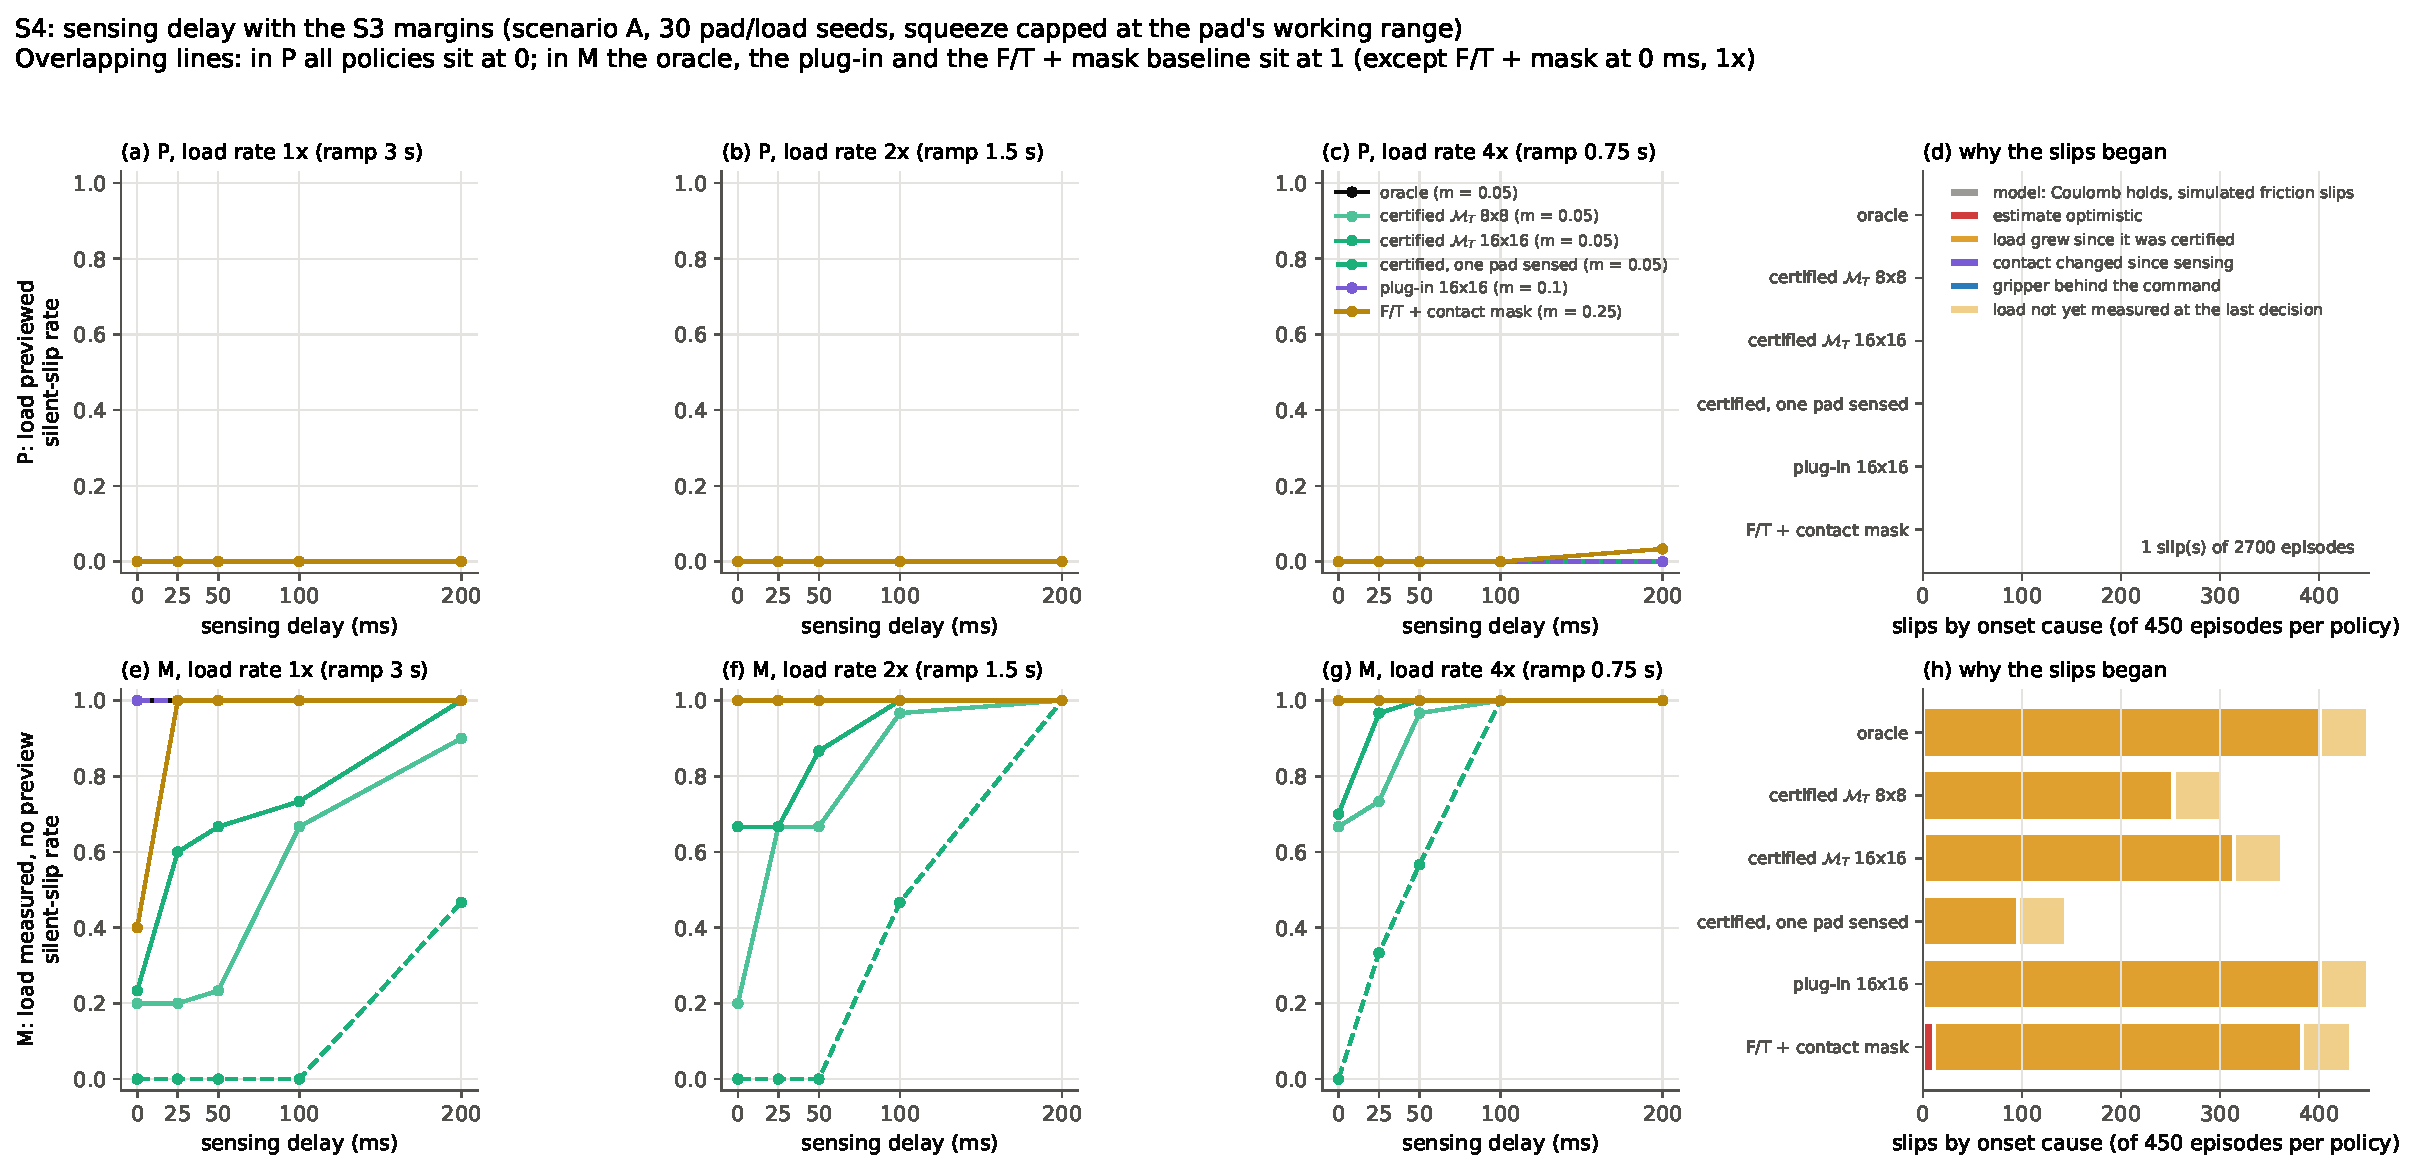
\includegraphics[width=\linewidth]{delay_envelope.pdf}
\caption{S4. Silent-slip rate against the sensing delay with the S3 margins; top row: load previewed (P), bottom row: load measured (M); columns:
load rate $1\times$, $2\times$, $4\times$; right: onset cause of every slip.}
\label{fig:S4}
\end{figure}

\begin{itemize}
    \item \textbf{Causes.} Of the 2142 slips in mode M, 1836 are \emph{load} (the load grew since the one certified), 294 \emph{load not yet measured},
    11 \emph{estimate} (contact mask), 1 \emph{model}, and none \emph{state} or \emph{actuator}. The median capacity / demand at onset is 0.75.
    \item \textbf{When.} The slips begin at load onset, at a fixed point of the ramp for every method and delay: 13\% into the 3\,s ramp, 20\% into
    the 0.75\,s ramp. They are real slips of 2--5\,mm (median 2.6\,mm), not boundary ticks. The episode in Figure~\ref{fig:S4episode} slipped early and
    then held; recovery was not checked systematically.
    \item \textbf{Why the oracle fails at $\Delta=0$.} Without preview, the load keeps growing during the 50\,ms command hold and the gripper lag. Early
    in a ramp from zero this growth is large in relative terms, about one control period divided by the elapsed time per cycle (13\% at 0.39\,s),
    which exceeds the multiplicative margin $m=0.05$.
    \item \textbf{Certificates survive in proportion to their conservatism.} The median estimate term at onset is $-0.88$ (one pad), $-0.30$
    ($8\times8$), $-0.15$ ($16\times16$) and about 0 (oracle, plug-in): the order of survival.
\end{itemize}

\begin{figure}[tbp]
\centering
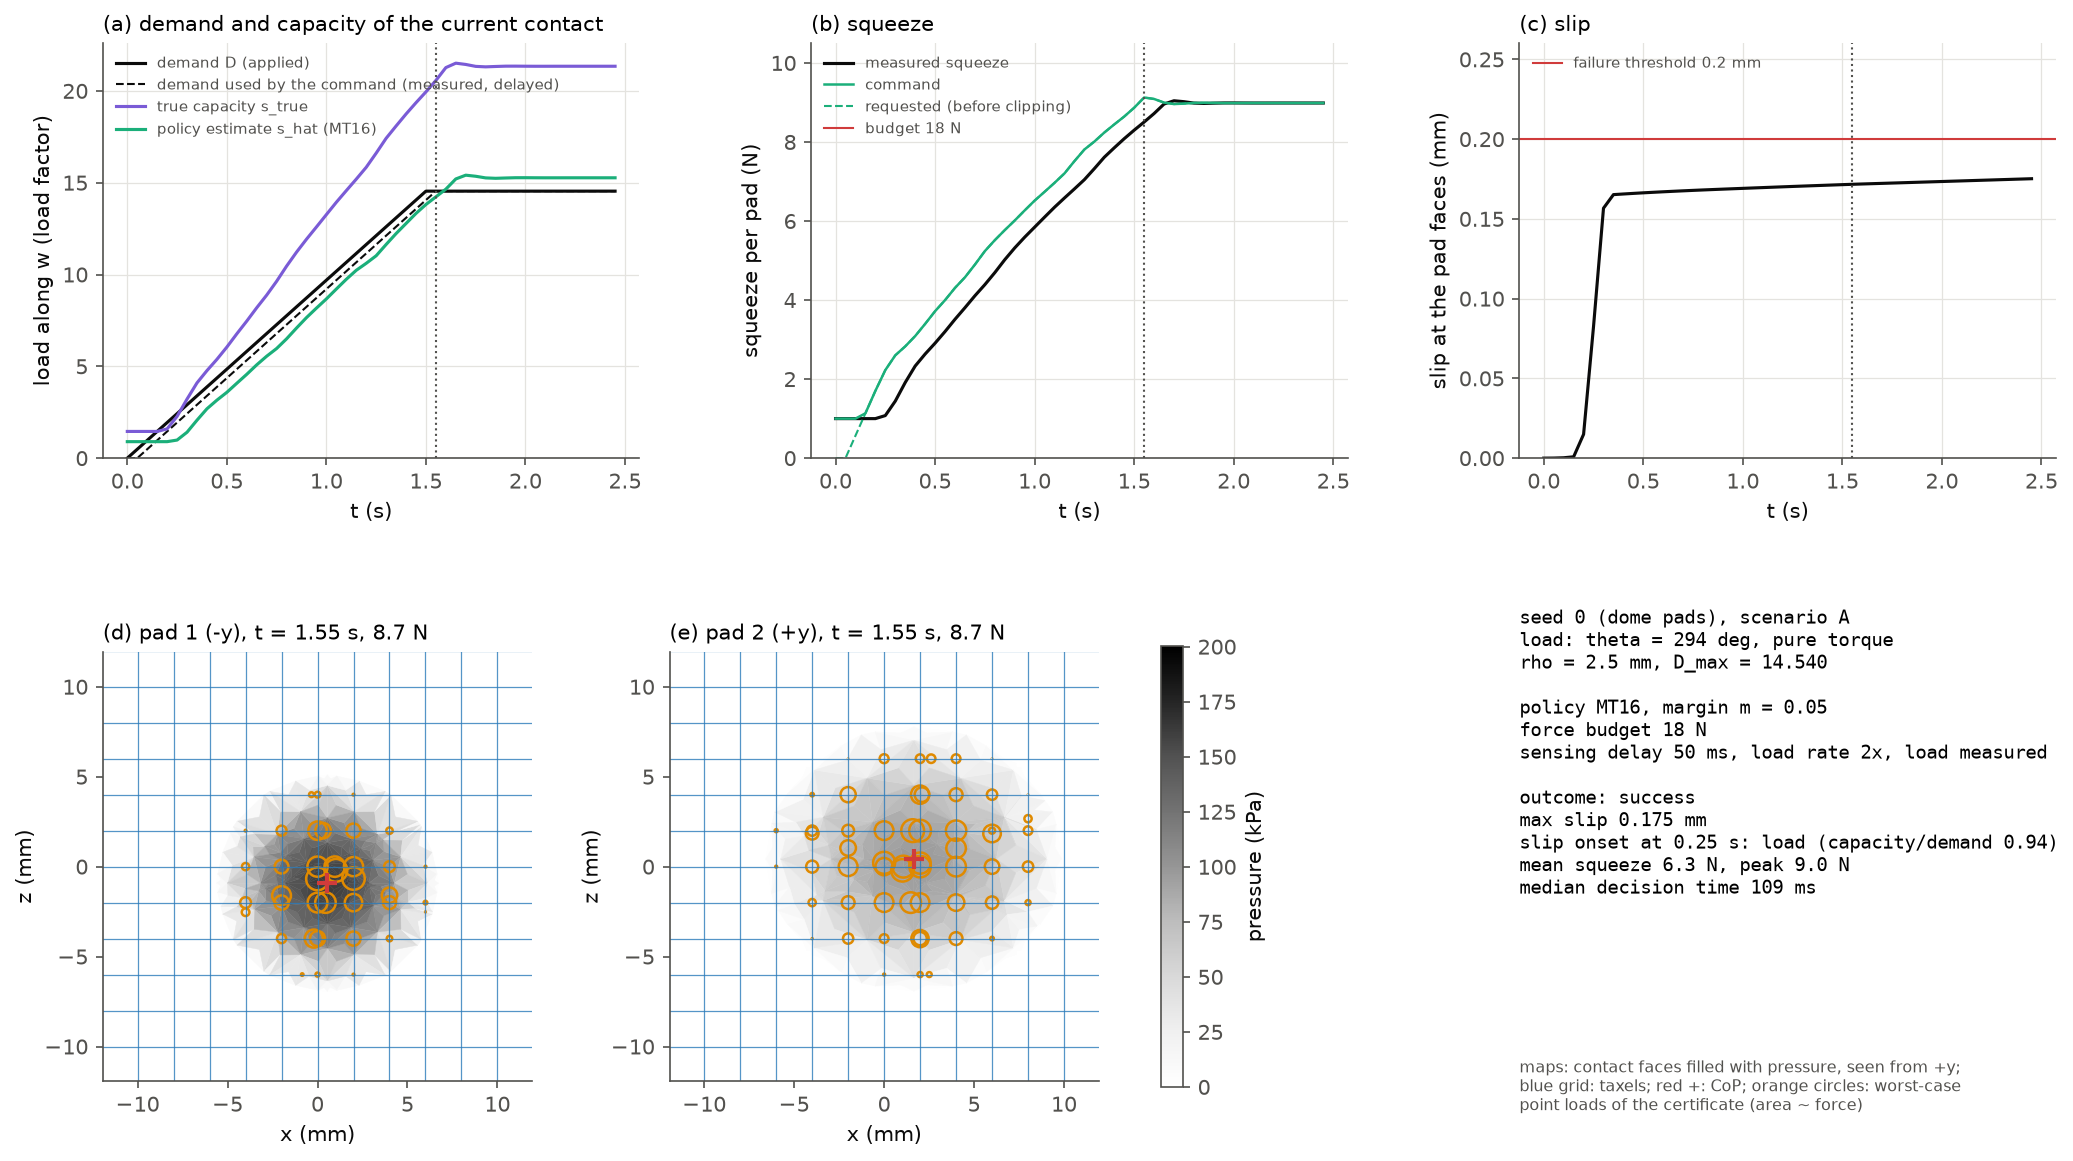
\includegraphics[width=\linewidth]{s4_episode.png}
\caption{S4, one episode in mode M ($\M_T$ $16\times16$, seed 0, $\Delta=50$\,ms, rate $2\times$; \code{sim-show -{}-delay 50 -{}-rate 2 -{}-no-preview}). (a) The
measured demand lags the applied demand, and the true capacity dips below it at the start of the ramp; (c) the bar slips by 0.17\,mm at load
onset, just under the failure threshold, then holds once the squeeze catches up. Slip onset at 0.25\,s, cause \emph{load}, capacity / demand 0.94.}
\label{fig:S4episode}
\end{figure}

\paragraph{Interpretation.}
\begin{itemize}
    \item \textbf{The weak link is temporal, not the certificate}, as predicted. Delaying the tactile state costs nothing; not knowing the load ahead
    breaks every method, the oracle first.
    \item \textbf{The dynamic margin calibrated with preview does not transfer to a measured load.} $m_{\rm dyn}=0.05$ covered the loop with preview
    only.
    \item \textbf{Conservatism acts as an implicit temporal margin.} This is conservatism, not a merit of certification: the guarantee concerns the
    sensed state, $w(t-\Delta)\in\X^-(y(t-\Delta))$, and says nothing about $w(t)$.
    \item \textbf{A static certificate needs a separate temporal term} covering the load change over the delay plus the loop lag. For a ramp from
    zero it cannot be a multiplicative margin, since the relative growth is unbounded at onset; it must be a load preview, an additive or
    rate-based term on the certified load (e.g.\ $D+\dot D\,L$ for a lag $L$), or a squeeze floor sized for the first cycles. None of these was
    implemented: the study stops at the requirement.
    \item This matches the observation of \citet[§V-C]{costanzo2020two} that static limit-surface control alone slips under fast load changes, here
    with the mechanism isolated.
\end{itemize}

% =====================================================================================================
\section{Synthesis}
\label{sec:synthesis}

\begin{table}[tbp]
\centering\small
\begin{adjustbox}{max width=\linewidth}\begin{tabular}{@{}p{0.36\linewidth}p{0.32\linewidth}p{0.24\linewidth}@{}}
\toprule
Claim & Evidence & Status \\
\midrule
F/T + CoP never certifies torsion about the CoP & Cor.~\T{cor:coarse_inner}; F1; S3 (uniform over pad fails at $m=1$) & proven; illustrated \\
Exact, tractable taxel bounds ($\M_F$ closed form, $\M_T$ SOCP/LP) & Thms~\T{thm:MF}, \T{thm:combined_lower}, \T{thm:combined_upper}; verification & proven; verified \\
Certified and upper load factors, tight, multi-contact; hold / slip / undecided & Prop.~\T{prop:load_factor}; tests; load factor; S2 & proven (sketch); verified \\
Gap halves per dyadic refinement; value of the CoP for mixed loads & Props.~\T{prop:taxel_refinement}--\T{prop:taxel_resolution_MT}, Thm~\T{thm:rate}; F2; load factor; S3 & proven; quantified \\
Plug-in estimates are unsafe & F3; load factor; S3 & numerical, simulation \\
Certificate sound in closed loop; price & S3 & simulation (Drake, planar joint) \\
Value is robustness, not efficiency & S3 tuned-margin transfer & simulation \\
Static certificate needs a temporal term & S4 & simulation \\
Coulomb patch model holds on a gel & --- & open (hardware) \\
Robust bounds under taxel noise & --- & open (theory) \\
\bottomrule
\end{tabular}\end{adjustbox}
\caption{Claims and the evidence in this report.}
\label{tab:synthesis}
\end{table}

\paragraph{Limitations.}
\begin{itemize}
    \item Planar, quasi-static Coulomb friction with a known, uniform $\mu$, and noise-free taxel forces.
    \item The closed-loop results use a planar joint for the bar (out-of-plane moments carried without friction) and Drake's lagged solver with a tight
    stiction tolerance; other settings change the outcome (S2).
    \item The controller's linear scaling of capacity with squeeze, its relaxation limit and the load preview are heuristics outside the theory.
    \item The dynamic margin is calibrated on the oracle in one loop; it is a property of the loop, not of the certificate.
    \item Simulated pads are hydroelastic: their pressure comes from penetration depth, not elasticity; they serve as test fields, not as a model of a
    gel.
\end{itemize}

% =====================================================================================================
\section{Planned work}
\label{sec:planned}
The outcomes of the following studies are open; this section states what they will test.

\subsection{Robust extension}
\label{sec:robust}
\paragraph{Motivation.} Real taxel forces are noisy, and vision-based tactile sensors provide pressure only through an elastic reconstruction, so the
measurement is an interval rather than a value. The friction coefficient is also uncertain.
\paragraph{Theory.} Bounds and the certified load factor for interval taxel forces $F_i\in[F_i^-,F_i^+]$ (with consistent totals and, for $\M_T$, a
convex set of CoPs) and $\mu\in[\mu_{\rm lo},\mu_{\rm hi}]$. The friction coefficient only scales the bounds. For a fixed twist, the $\M_T$ lower
bound stays an SOCP with interval taxel forces, since it is jointly convex in the forces and the local first moments (Theorem~\T{thm:combined_lower}).
For the load factor, the twist is a variable and $F_i$ multiplies the direction $a$, so the substitution $u_i=bc_i$ of Proposition~\T{prop:load_factor}
may not keep the problem jointly convex; another formulation or a relaxation with a certified gap may be needed.
\paragraph{Numerical study (F4: resolution against noise).} Pixel noise aggregated into taxel intervals. The nominal gap shrinks like $1/k$
(Proposition~\T{prop:taxel_resolution_MT}) while the sum of the interval widths grows like $\sqrt r$ for $r=k^2$ independent taxels, so an interior
optimal resolution is plausible; the study will test whether it exists and where.
\paragraph{Simulation.} Repeat S3 with noisy taxels and the robust certificate, to test whether soundness survives and at what cost.

\subsection{Hardware validation}
\label{sec:hardware}
\paragraph{Purpose.} The only independent physical test: does the Coulomb patch model, which the certificate assumes, hold on a real sensor gel?
\citet[§3]{howe1996practical} report that silicone and rubber fingertips slip below the Coulomb limit-surface prediction under combined torsion and
shear, so soundness is not presumed; the study is a \emph{model-adequacy test}, and violations will be reported.
\paragraph{Set-up.} No gripper. A GelSight Mini is mounted on a six-axis ATI force/torque sensor at the robot wrist. The ATI gives the full contact
wrench at 1\,kHz, hence $f_N$ and the CoP exactly (the $\M_0$ information). The GelSight supplies only the \emph{shape} of the normal-force distribution.
Objects touch the gel through small flat-topped bosses, so that the whole contact stays inside the field of view.
\paragraph{Calibration.}
\begin{itemize}
    \item \textbf{Pressure from depth.} The depth map is mapped to pressure inside the contact mask, integrated over $k\times k$ cells and scaled to the
    ATI's $f_N$. A local depth--pressure law is only a first approximation for a nearly incompressible gel, so the map is calibrated with statically
    determinate indenters: one to three bosses whose individual forces follow exactly from the ATI's force and moments. It is validated on held-out
    shapes against the ATI CoP. Its residuals give the taxel intervals of the robust extension.
    \item \textbf{Friction coefficient.} $\mu$ comes from pure-shear slides only, since translational capacity is $\mu f_N$ for any pressure
    \citep[§2.3]{howe1996practical}. Torsion and combined loads are held out as the test. The calibration records the dependence on normal force,
    speed and dwell time, and the drift.
\end{itemize}
\paragraph{Model-adequacy tests (single contact, indenter clamped to the table).} T1: steady sliding at an imposed twist $q$, set by the instantaneous
centre of rotation. Maximum dissipation gives $\langle w_{\rm meas},q\rangle=h(q)$, with the wrench and the twist written about the same point (the ATI reference),
which is compared with $[\underline h(q),\overline h(q)]$ for $\M_0$, $\M_F$ and $\M_T$ at each resolution. T2: a tangential wrench ramped along a fixed $w$ until gross slip, with $s_{\rm obs}$ compared with $[\underline s,\overline s]$, as
in S2. The plug-ins, the contact-mask method and the parametric model of \citet{costanzo2020two} are evaluated on the same frames. Short slides with
filleted bosses and an automatic abort protect the gel.
\paragraph{Demonstrations.}
\begin{itemize}
    \item \textbf{Dial (single contact).} The sensor turns a spring-loaded dial through friction, with the certified minimal press force under a pure
    torsional load that rises with the angle. This is a previewed load, mode P of S4.
    \item \textbf{D1.} A plate is held between the GelSight and a passive pad on a vertical bar while a container at a lever arm fills slowly. This is the
    hardware counterpart of S3/S4 scenario A, with the load either previewed (known flow) or measured.
    \begin{itemize}
        \item Configuration V: the passive side has low friction, so the ATI measures the whole tangential load.
        \item Configuration D: the passive side is a gel, with the load split measured as a side result.
    \end{itemize}
\end{itemize}
Methods: F/T only, which cannot certify torsion; plug-ins; contact mask; parametric; certified at $2\times2$ to $16\times16$. Metrics: slip, flags, peak
squeeze.
\paragraph{What the simulations imply for the design.}
\begin{itemize}
    \item With a measured load, the loop must certify the load growth over the measured latency (S4), or use a previewed load.
    \item A free object with offset normal-force centres loads friction out of plane (S3). Coaxial bosses and a load hung in the mid-plane avoid it.
    \item An unsensed contact is costly (2.4 times the oracle squeeze in S3). In configuration D its worst case is taken over the known boss face only.
\end{itemize}
A gate on recorded maps of the demo objects (certified gap of at least 1.5 between $2\times2$ and $16\times16$, forces within the gel's limit) precedes
the demonstrations. The detailed protocol and phases are in \code{research/stage3\_validation\_plan.md}, §9.

% =====================================================================================================
\appendix
\section{Reproducibility}
\label{sec:repro}
\begin{table}[H]
\centering\small
\begin{adjustbox}{max width=\linewidth}\begin{tabular}{@{}lll@{}}
\toprule
Study & Command (\code{pixi run \dots}) & Cache / output \\
\midrule
Tests & \code{test} & --- \\
Verification & \code{counterexample}, \code{bounds}, \code{refinement} & \code{examples/figures/} \\
Field population, F1 & \code{fields}, \code{wrench-sets} & \code{doc/figures/fields.pdf}, \code{wrench\_sets.pdf} \\
F2, F3 & \code{resolution}, \code{plugin} & \code{examples/data/study.npz} \\
Load factor & \code{load-factor} & \code{doc/figures/load\_factor.pdf} \\
S1 & \code{-e sim sim-smoke} & \code{sim/out/smoke.*} \\
S2 & \code{-e sim sim-sweep} & printed table \\
S3 & \code{-e sim sim-grip}, \code{sim-grip-plot} & \code{sim/data/grip\_study\_v2.npz} \\
S4 & \code{-e sim sim-delay}, \code{sim-delay-plot} & \code{sim/data/delay\_study.npz} \\
One episode & \code{-e sim sim-show -{}-seed 0 -{}-policy MT16 [-{}-delay 50 -{}-rate 2 -{}-no-preview]} & \code{sim/out/episode\_*} \\
\bottomrule
\end{tabular}\end{adjustbox}
\caption{Commands, run from the root of the code repository \code{pfb}; vector figures are written to \code{\$PFB\_DOC\_FIG}
(\code{make figures} in this repository sets it to \code{doc/figures/}). Drake runs in the pixi environment \code{sim}.}
\end{table}
Settings: Drake discrete solver \emph{lagged}, stiction tolerance $10^{-6}$\,m/s, time step 1\,ms, control period 50\,ms, gripper filter 50\,ms, load
and filter update 5\,ms, $\mu=0.8$, slip threshold 0.2\,mm at the pad faces. Seeds 0--29 cycle through the pad families (dome, tilted, flat). S3: 1.8\,h,
S4: about 1\,h, on 22 processes.
\IfFileExists{code_version.tex}{\input{code_version.tex}\par\noindent Figures and numbers built against code commit \code{\codeversion}.}{}

\bibliographystyle{plainnat}
\bibliography{references}

\end{document}
